\documentclass[10pt,b5paper,openright]{book}
\usepackage{packages}

\begin{document}

% Roman numbering for the front matter
\pagenumbering{roman} 

% TODO: No problem description?
%\section*{\Huge{Problem Description}}
%\addcontentsline{toc}{chapter}{Problem Description}
%\input{./chapters/problem_description}
%\newpage

\section*{\Huge{Abstract}}
\addcontentsline{toc}{chapter}{Abstract}
\Glspl{uvms} are increasingly utilized for complex underwater tasks, including inspection, mapping, maintenance, and repair.
Typical operations require managing multiple simultaneous objectives, such as controlling the position and orientation of an end-effector while maintaining optimal viewpoints from cameras and lighting systems mounted elsewhere on the \gls{uvms}.
Additionally, light-\glspl{uvms} pose unique control challenges due to significant coupling between the base vehicle and its manipulator arm, rendering decoupled control approaches less effective.

A promising solution to address these challenges is \gls{tpc}, an approach that allows explicit prioritization of tasks according to their relative importance. This thesis explores the application of \gls{tpc} to \glspl{uvms}, focusing specifically on the practical implementation and evaluation of kinematic-level \gls{tpc} frameworks.

This thesis contributes to the experimental verification of a \gls{tpc} framework by developing a dedicated C++ control library for the Eelume robot—a highly coupled, high-\gls{dof}, light-\gls{uvms}. The library includes a built-in simulator and supports both development and deployment of control strategies.

Experiments conducted in the Trondheim fjord as part of the thesis demonstrate the efficacy of kinematic-level \gls{tpc} when applied to \glspl{uvms}.
These results not only validates the practical applicability of kinematic-level \gls{tpc} but also lays a robust foundation for future research into dynamic-level \gls{tpc} and the exploration of alternative advanced control strategies using the Eelume robot.


\newpage

\section*{\Huge{Sammendrag}}
\addcontentsline{toc}{chapter}{Sammendrag}
Undervanns farkost-manipulator systemer (UVMSs) brukes i økende grad til komplekse undervannsoppgaver som inspeksjon, kartlegging, vedlikehold og reparasjon. Slike operasjoner innebærer ofte at man må håndtere flere samtidige mål, for eksempel å kontrollere posisjonen og orienteringen til manipulator-armen, samtidig som man opprettholder gode synsvinkler fra kameraer og lys montert andre steder på UVMS-en.

I tillegg byr lette UVMS-er på særegne kontrollutfordringer på grunn av sterk kobling mellom basen og manipulatorarmen, noe som gjør at tradisjonelle, separerte kontrollmetoder blir mindre effektive.

En lovende tilnærming for å håndtere disse utfordringene er Task-Priority Control (TPC), en metode som tillater eksplisitt prioritering av kontrolloppgaver basert på deres relative viktighet. Denne oppgaven undersøker anvendelsen av TPC for UVMS-er, med særlig fokus på praktisk implementering og evaluering av TPC-rammeverk på kinematisk nivå.

Som et bidrag til eksperimentell validering av et TPC-rammeverk, utvikles et dedikert C++ kontrollbibliotek for Eelume-roboten—en sterkt koblet, slangelignende undervannsrobot med mange frihetsgrader. Biblioteket inkluderer en innebygd simulator og støtter både utvikling og utprøving av kontrollstrategier.

Eksperimenter gjennomført i Trondheimsfjorden som en del av arbeidet viser at TPC på kinematisk nivå fungerer effektivt når det anvendes på UVMS-er. Resultatene bekrefter ikke bare den praktiske anvendbarheten av metoden, men legger også et solid grunnlag for videre forskning på TPC på dynamisk nivå og utforskning av alternative avanserte kontrollstrategier med Eelume-plattformen.

\newpage

\section*{\Huge{Preface}}
\addcontentsline{toc}{chapter}{Preface}
This thesis was created as part of my Master's at the Norwegian University of Science and Technology (NTNU) in Trondheim, Norway, during the spring of 2025. It completes the five-year Master's program in Cybernetics and Robotics at the Faculty of Information Technology and Electrical Engineering.

This thesis is a continuation of my project thesis, "Task-Priority Control of Underwater Vehicle-Manipulator Systems", written in the autumn of 2024. As such, some parts of this thesis are based primarily on the work done in that project. The sections in \autoref{sec:background} are based on the project thesis, except for \autoref{sec:background:quaternions}, which was added to provide some context for the quaternion-based dynamic model and control laws. The sections in \autoref{chap:modeling} are also based on the project thesis but include changes related to incorporating quaternions into the model. \autoref{chap:tpc} has been rewritten to better align with the standard representation of kinematics and dynamics of \gls{uvms}s as presented in the literature.

Finally, I would like to thank my co-supervisors, Markus H. Iversflaten and Bjørn K. Sæbø, for all their help and support during the project. Many days were spent together conducting experiments at Trondheim Biological Station, and I am very grateful for all the time they devoted to assisting me.

\DTMlangsetup{showdayofmonth=false}
\begin{flushright}
    \textit{Håkon Bårsaune} \\
    \textit{Trondheim,\today}
\end{flushright}
\DTMlangsetup{showdayofmonth=true}
\newpage


\tableofcontents
\newpage

% List of figures and tables, they don't need take two pages each
\begingroup

\let\cleardoublepage\relax
\let\clearpage\relax
\listoffigures
\addcontentsline{toc}{chapter}{List of Figures}

\newpage
\listoftables
\addcontentsline{toc}{chapter}{List of Tables}

%\newpage
%\lstlistoflistings

\newpage
\printglossary[type=\acronymtype]
\addcontentsline{toc}{chapter}{List of Acronyms}

\endgroup


\newpage


\chapter{Introduction}
\pagenumbering{arabic} % Arabic numbering for the main matter
% Change the page style to include the chapter number and title in the header
\fancyhead[RE]{\thepage}
\fancyhead[LE]{\MakeUppercase{\rightmark}}
\fancyhead[LO]{\thepage}
\fancyhead[RO]{\MakeUppercase{\leftmark}}
\fancyfoot[C]{}

%\chapter{Introduction}
\section{Motivation}
\section{Contribution}
\section{Thesis Outline}
\section{Literature Review}

\chapter{Background and {Preliminaries}}
\label{sec:background}

% -----------------------------------------------------------------------------
\section{Special Orthogonal Group in 3 dimensions}
\label{sec:bp:so3_se3}

The special orthogonal group in three dimensions, $\SO$, and the special
Euclidean group in three dimensions, $\SE$, are key mathematical tools in the
study of rigid body dynamics. These groups serve distinct purposes: $\SO$ is
used to represent rotations, while $\SE$ describes rigid body and spatial
transformations. This section offers a brief introduction to these groups and
highlights some of their essential properties.

We denote by $\SO$ the special orthogonal group in three dimensions, which is
the group of all $3 \times 3$ rotation matrices with determinant equal to one,
such that
\begin{align}
    \SO = \{ \bm{R} \in \mathbb{R}^{3 \times 3} \mid \bm{R}^T \bm{R} = \mathbb{I}, \det(\bm{R}) = 1 \}.
\end{align}
Intuitively, $\bm{R}^T \bm{R} = \mathbb{I}$ means that the columns of $\bm{R}$ are orthonormal,
and $\det(\bm{R}) = 1$ means that $\bm{R}$ is a proper rotation, i.e., it does not include
a reflection. The $\SO$ group is closely related to the Lie algebra $\so$
\begin{subequations}
\begin{align}
    \so &= \{ \bm{\Omega} \in \R^{3 \times 3} | \bm{\Omega}^T = -\bm{\Omega} \} \\
    [\bm{\Omega_1}, \bm{\Omega_2}]_{\so} &= \bm{\Omega_1} \bm{\Omega_2}
        - \bm{\Omega_2} \bm{\Omega_1},
\end{align}
\end{subequations}
by the exponential map
\begin{subequations}
\begin{align}
    \exp &: \so \to \SO \\
    \exp &: \bm{\Omega} \mapsto \sum_{k=0}^{\infty} \frac{1}{k!} \bm{\Omega}^k.
\end{align}
\end{subequations}
This is an important property, as it is fundamental to the definition of the
angular velocity $\bm{\omega}$ of a rigid body. Consider a rotation matrix
$\bm{R}_b^i$ that rotates a vector from the body-fixed frame $b$ to some inertial
frame $i$. The body-fixed angular velocity $\bm{\omega}_{ib}^b$ is then defined
as
\begin{align}
    \cross{\bm{\omega}_{ib}^b} = \bm{R}_i^b \dot{\bm{R}}_b^i.
\end{align}
When specifying reference frames, we say that
\begin{align}
    \bm{p}^b = \bm{R}_{a}^b \bm{p}^a,
\end{align}
meaning that the rotation matrix $\bm{R}_{a}^b$ rotates a vector
$\bm{p}^a\in\R^3$ from frame $a$ to frame $b$. Some important properties
of $\bm{R}_a^b \in \SO$ are as follows \cite{modsim}:
\begin{itemize}
\item $\bm{R}_a^b = (\bm{R}_b^a)^{-1} = (\bm{R}_b^a)^T$
\item $\bm{R}_a^b \bm{R}_b^c = \bm{R}_a^c$.
\end{itemize}

Rotations in three-dimensional space can be parameterized using various methods,
including Euler angles, quaternions, angle-axis representations, and
Rodrigues parameters. In this thesis, Euler angles are used for simplicity.
Euler angles are a set of three angles that describe a sequence of three
rotations about the principal axes of a reference frame. These rotations are
performed in a specific order: typically about the $x$-axis, followed by the $y$
-axis, and finally the $z$-axis. The resulting transformation is represented by
a rotation matrix $\bm{R}$, which encodes the cumulative effect of these three
successive rotations.
Explicitly, if the three Euler angles are denoted as $\phi$, $\theta$, and $\psi$,
corresponding to rotations about the $x$-, $y$-, and $z$-axes respectively,
the rotation matrix is given by \cite{modsim}:
\begin{align}
    \bm{R} = \bm{R}_z(\psi) \bm{R}_y(\theta) \bm{R}_x(\phi),
\end{align}
where
\begin{subequations}
\label{eq:bp:so3:rotations}
\begin{align}
    \bm{R}_x(\phi) &= \begin{bmatrix}
        1 & 0 & 0 \\
        0 & \cos\phi & -\sin\phi \\
        0 & \sin\phi & \cos\phi
    \end{bmatrix}, \\
    \bm{R}_y(\theta) &= \begin{bmatrix}
        \cos\theta & 0 & \sin\theta \\
        0 & 1 & 0 \\
        -\sin\theta & 0 & \cos\theta
    \end{bmatrix}, \\
    \bm{R}_z(\psi) &= \begin{bmatrix}
        \cos\psi & -\sin\psi & 0 \\
        \sin\psi & \cos\psi & 0 \\
        0 & 0 & 1
    \end{bmatrix}.
\end{align}
\end{subequations}
A disadvantage of using Euler angles is the well known problem of gimbal lock.
This occurs when two of the three axes align, causing the rotation matrix to
lose a degree of freedom. We say that the system has lost a degree of freedom
when this happens. In practice it is often possible to avoid this issue by not
controlling the system to a $\pm90^\circ$ pitch angle, or by switching to a
different angle representation when the system approaches gimbal lock. In this
work we avoid this issue by not controlling the system to these singularities.

% -----------------------------------------------------------------------------
\section{Special Euclidean Group in 3 dimensions}
\label{sec:bp:se3}

The special Euclidean group in three dimensions, $\SE$, is the group of all
rigid body transformations in three-dimensional space. It is defined as
\begin{align}
    \SE := \left\{ \begin{bmatrix}
        \bm{R} & \bm{p} \\
        \bm{0} & 1
    \end{bmatrix}
        \in \R^{4 \times 4} \middle| \bm{R} \in \SO, \, \bm{p} \in \R^3
    \right\}.
\end{align}
A transformation by 
\begin{align}
    \bm{T}_b^i = \begin{bmatrix}
        \bm{R}_{b}^i & \bm{p}_{ib}^i \\
        \bm{0} & 1
    \end{bmatrix}
\end{align}
will operate on a vector $\bm{p}_{bo}^b \in \R^3$:
\begin{align}
    \begin{bmatrix}
        \bm{p}_{io}^i  \\
        1
    \end{bmatrix}
    =
    \bm{T}_b^i \begin{bmatrix}
        \bm{p}_{bo}^b \\
        1
    \end{bmatrix}
    =
    \begin{bmatrix}
        \bm{R}_{b}^i \bm{p}_{bo}^b + \bm{p}_{ib}^i \\
        1
    \end{bmatrix}.
    \label{eq:se3_transformation}
\end{align}
One can intuitively see from \autoref{eq:se3_transformation} that the transformation
$\bm{T}_b^i$
takes a vector $\bm{p}_{bo}^b$, the vector from the body-origin $b$ to the point $o$
in the $b$ frame, and transforms it to the vector $\bm{p}_{io}^i$, the vector from
the inertial-frame origin $i$ to the point $o$ described in the $i$ frame.


Consider an element $\bm{H}_{b}^i \in \SE$, which is a transformation from frame
$b$ to frame $i$. The body-fixed twist $\bm{\nu}_{ib}^b$ and the inertial-frame
twist $\bm{\nu}_{ib}^i$ are defined respectively as
\begin{subequations}
\begin{align}
    [\bm{\nu}_{ib}^b]_{\wedge} &= \left(\bm{H}_{b}^i\right)^{-1}\dot{\bm{H}}_{b}^i \label{eq:body_twist_def}\\
    [\bm{\nu}_{ib}^i]_{\wedge} &= \dot{\bm{H}}_{b}^i \left(\bm{H}_{b}^i\right)^{-1}. 
\end{align}
\end{subequations}

Similar to $\SO$, the Lie algebra $\se$ is closely related to $\SE$ by the exponential
map. The Lie algebra $\se$ is defined as
\begin{subequations}
    \label{eq:se3_algebra}
\begin{align}
    \se &= \left\{ \begin{bmatrix}
        \bm{\Omega} & \bm{v} \\
        \bm{0} & 0
    \end{bmatrix}
    \in \R^{4 \times 4}
    \middle|
    \bm{\Omega} \in \so, \, \bm{v} \in \R^3
    \right\} \\
    \left[ \Gamma_1, \Gamma_2 \right]_{\se} &= \Gamma_1 \Gamma_2 - \Gamma_2 \Gamma_1 \\
    \exp &: \se \to \SE
\end{align}
\end{subequations}
We define the matrix representation of the ad-operator
\begin{align}
    \ad_{\se} : \R^6 \to \R^{6 \times 6},
\end{align}
implicitly by requiring that for all $\bm{y} \in \R^6$
\begin{align}
    \ad_{\se}( \bm{x} ) \bm{y} = \bm{x} \wedge \bm{y}. \label{eq:ad_impl}
\end{align}
The resulting $\ad_{\se}(\bm{x})$ matrix is then
\begin{align}
    \ad_{\se} : \begin{bmatrix} \bm{v} \\ \bm{\omega} \end{bmatrix}
        \mapsto \begin{bmatrix}
            [\bm{\omega}]_{\times} & [\bm{v}]_{\times} \\
            \bm{0} & [\bm{\omega}]_{\times}
        \end{bmatrix}.
\end{align}
In a similar fashion, the matrix representation of the $\Ad$ operator
\begin{align}
    \Ad_{\SE} : \SE \to \R^{6 \times 6}
\end{align}
is defined. This operator is implicitly defined by requiring that for all
$\bm{\nu} \in R^6$, $\bm{H} \in \SE$
\begin{align}
    [\Ad_{\SE}(\bm{H})\bm{\nu}]_{\wedge} = \bm{H} [\bm{\nu}]_{\wedge} \bm{H}^{-1}.
\end{align}
This is essentially a mapping from body-fixed twists to inertial-frame twists,
and is extensively used when modeling UVMs. The $\Ad$-operator is then
\begin{align}
    \Ad_{\SE} : \begin{bmatrix}
        \bm{R} & \bm{p} \\
        \bm{0} & 1
    \end{bmatrix}
    \mapsto
    \begin{bmatrix}
        \bm{R} & [\bm{p}]_{\times} \bm{R} \\
        \bm{0} & \bm{R}
    \end{bmatrix}.
\end{align}
The $\Ad$ operator of the inverse of an element of $\SE$ is also widely used
\begin{subequations}
\begin{align}
    \Ad_{\SE}^{-1} &: \begin{bmatrix}
        \bm{R} & \bm{p} \\
        \bm{0} & 1
    \end{bmatrix}
    \mapsto
    \begin{bmatrix}
        \bm{R}^T & - \bm{R}^T [\bm{p}]_{\times} \\
        \bm{0} & \bm{R}^T
    \end{bmatrix} \\
    \Ad_{\SE}^{-1}(\bm{H}) &= \Ad_{\SE}(\bm{H}^{-1}).
\end{align}
\end{subequations}
In the following chapters, the $\ad$- and $\Ad$-operators will always refer to
the $\se$ and $\SE$ Lie algebras and groups, respectively.

% -----------------------------------------------------------------------------
\section{Pseudo-Inverse and Null Space Projections}
\label{sec:pseudoinverse}

For a given matrix $\bm{A} \in \mathbb{R}^{n\times m}$ we define the Moore-Penrose
pseudo-inverse $\bm{A}^{+} \in \mathbb{R}^{m\times n}$ as the unique matrix
satisfying the following four properties \cite{penrose1955}:
\begin{subequations}
    \begin{align}
        &\textrm{1. } & \bm{A}\bm{A}^{+}\bm{A} &= \bm{A} \\
        &\textrm{2. } & \bm{A}^{+}\bm{A}\bm{A}^{+} &= \bm{A}^{+} \\
        &\textrm{3. } & (\bm{A}\bm{A}^{+})^T &= \bm{A}\bm{A}^{+} \\
        &\textrm{4. } & (\bm{A}^{+}\bm{A})^T &= \bm{A}^{+}\bm{A}
    \end{align}
\end{subequations}
Note that in the general case, the transpose operator can be replaced by the
conjugate transpose (hermitian) operator for matrices over the complex field $\mathbb{C}$ \cite{penrose1955}.
It can be shown that for a full-column rank matrix $\bm{A}$, the pseudo-inverse is
\begin{align}
    \bm{A}^{+} = (\bm{A}^T \bm{A})^{-1} \bm{A}^T,
\end{align}
and for a full-row rank matrix $\bm{A}$, the pseudo-inverse is
\begin{align}
    \bm{A}^{+} = \bm{A}^T (\bm{A} \bm{A}^T)^{-1}.
\end{align}
In the general case, whether or not $\bm{A}$ is full rank, the pseudo-inverse can always
be computed using the singular value decomposition (SVD) of $\bm{A}$. The SVD of $\bm{A}$ is
\begin{subequations}
\begin{align}
    \bm{A} &= \bm{U} \bm{\Sigma} \bm{V}^T \\
    \bm{U} &\in \mathbb{R}^{n\times n} \textrm{ unitary} \\
    \bm{V} &\in \mathbb{R}^{m\times m} \textrm{ unitary} \\
    \bm{\Sigma} &= \operatorname{diag}(\sigma_1, \sigma_2, \ldots, \sigma_r, 0, \ldots, 0) \in \mathbb{R}^{n\times m} \\
    \sigma_1 &\geq \sigma_2 \geq \ldots \geq \sigma_r > 0 \\
    r &= \operatorname{rank}(\bm{A}).
\end{align}
\end{subequations}
Where a matrix $U$ is unitary if and only if $U^T U = U U^T = \mathbb{I}$. The pseudo-inverse
of $\bm{A}$ can then be computed as
\begin{subequations}
\begin{align}
    \bm{A}^{+} &= \bm{V} \bm{\Sigma}^{+} \bm{U}^T \\
    \bm{\Sigma}^{+} &:= \operatorname{diag}(\sigma_1^{-1}, \sigma_2^{-1}, \ldots, \sigma_r^{-1}, 0, \ldots, 0).
\end{align}
\end{subequations}
The singular value decomposition will be important when dealing with
singularity-robust task-priority control later on in this thesis.

Consider the optimization problem
\begin{align}
    \min_{\bm{x} \in \mathbb{R}^m} || \bm{A} \bm{x} - \bm{b} ||.
\end{align}
The solution to this problem is given by
\begin{align}
    \bm{x} = \bm{A}^{+} \bm{b} + (\mathbb{I} - \bm{A}^{+} \bm{A}) \bm{z},
\end{align}
where $\bm{z} \in \mathbb{R}^n$ is an arbitrary vector. The term $(\mathbb{I} - \bm{A}^{+} \bm{A}) \bm{z}$
is the null-space projection of $\bm{z}$ onto the null-space of $\bm{A}$. Parts
of this fact can bee seen by noting that
\begin{align}
    \bm{A}\left(\mathbb{I} - \bm{A}^{+} \bm{A}\right) = \bm{A} - \bm{A} = 0.
\end{align}
This is a fact that will be used extensively when formulating the task-priority
controllers in later chapters.

% -----------------------------------------------------------------------------
\section{Lagrange's Equation of Motion}
\label{sec:lagrange}
Lagrange's equation of motion is a formulation of the equations of motion of a
system in terms of generalized coordinates. The equations are derived from the
d'Alembert principle. It can be shown that the equations of motion derived from
Lagrange's equation are equivalent to the equations of motion derived from
the classical Newton-Euler equations \cite{modsim}. There are however some advantages to using
Lagrange's equation. For example, the equations are easier to derive for complex
systems where the kinetic and potential energy is known. With modern computer
algebra systems, the equations can be derived automatically, which is
a great advantage for complex systems.

Consider a system with $n$ generalized coordinates $q_1, q_2, \ldots, q_n$, and
their time derivatives $\dot{q}_1, \dot{q}_2, \ldots, \dot{q}_n$. Collect the
generalized coordinates in the vector $\bm{q} \in \mathbb{R}^n$ and the time
derivatives in the vector $\bm{\dot{q}} \in \mathbb{R}^n$. The kinetic energy
of the system is then a function $T$ of $\bm{q}$ and $\bm{\dot{q}}$
\begin{align}
    T = T(\bm{q}, \bm{\dot{q}})
\end{align}
and the potential energy is a function $U$ of $\bm{q}$
\begin{align}
    U = U(\bm{q}).
\end{align}
Define the lagrangian $L$ as the difference between the kinetic and potential
energy
\begin{align}
    L(\bm{q}, \bm{\dot{q}}) = T(\bm{q}, \bm{\dot{q}}) - U(\bm{q}).
\end{align}
The equations of motion are then given by \cite{modsim}:
\begin{align}
    \frac{d}{dt} \left( \nabla_{\dot{\bm{q}}} L \right) - \nabla_{\bm{q}} L = \bm{\tau},
\end{align}
where the $i$-th element of the vector $\bm{\tau}$ is the generalized force acting
on the $i$-th generalized coordinate. The generalized forces can be expressed as
\begin{align}
    \tau_i &= \sum_{k=1}^N \frac{\partial \bm{r}_k}{\partial q_i} \cdot \bm{F}_k
    & i &= 1, 2, \ldots,
\end{align}
where $\bm{r}_k$ is the position of the $k$-th force and $\bm{F}_k$ is the force
acting on this position. In cases where the kinetic energy is on the form
\begin{align}
    T = \frac{1}{2} \bm{\dot{q}}^T \bm{J}^T(\bm{q}) \bm{M} \bm{J}(\bm{q}) \bm{\dot{q}},
\end{align}
where $\bm{M}$ is symmetric and positive definite, the potential energy the
result of some potential field, and $\bm{J}(\bm{q})$ is the Jacobian of the
generalized coordinates, to be defined later, the equations of motion can be
written as
\begin{align}
    \bm{M}(\bm{q}) \ddot{\bm{q}} + \bm{C}(\bm{q}, \dot{\bm{q}}) \dot{\bm{q}} + \bm{g}(\bm{q}) = \bm{\tau}
\end{align}
where $\bm{M}(\bm{q})$ is symmetric and positive definite, $\bm{g}(\bm{q})$ is the
gradient of the potential field.

\section{Runge-Kutta Methods}
\label{sec:runge-kutta}

Runge-Kutta methods are a well-known set of numerical techniques used to solve
ordinary differential equations. They are popular because they are
straightforward to use and usually quite efficient. In this thesis, these
methods will be applied to model the dynamics of underwater vehicle-manipulator
systems, which can be described by ordinary differential equations.
When simulating controllers for these systems, it makes sense to use Runge
-Kutta methods, since they provide a convenient way to handle the required
calculations.

Consider a system of ordinary differential equations of the form
\begin{align}
    \dot{\bm{x}}(t) &= \bm{f}(\bm{x}(t), t) & \bm{x}(t_0) &= \bm{x}_0,
\end{align}
where $\bm{x}(t) : \R \to \R^n$ is the state of the system,
$\bm{f} : \R^n \times \R \to \R^n$ is a vector field, $t_0$ is the initial time,
and $\bm{x}_0$ is the initial state. In general, the solution to this system is
not known analytically, and numerical methods, such as Runge-Kutta must be used
to approximate the solution. These methods start by initializing the state to
$\bm{x}_0$ and then iteratively update the state using the vector field $\bm{f}$,
in time steps of size $h$. For explicit Runge-Kutta methods, the approximation
is given by \cite{modsim}:
\begin{subequations}
    \begin{align}
        \bm{k}_i &= \bm{f}(\bm{x}_n + h \sum_{j=1}^{i-1} a_{ij}\bm{k}_j, t_n + c_i h) &
            i &= 1, 2, \cdots, \sigma \\
        \bm{x}_{n+1} &= \bm{x}_n + h \sum_{i=1}^{\sigma} b_i \bm{k}_i,
    \end{align}
\end{subequations}
where $\{a_{ij}\}_{i,j}$, $\{b_i\}_i$, and $\{c_i\}_i$ are the coefficients of
the method, and $\sigma \in \mathbb{N}$ is the number of stages. The error $\bm{e}_{n+1}$ of
the method at time $t_{n+1}$ is given by
\begin{align}
    \bm{e}_{n+1} = \bm{x}_{n+1} - \bm{x}(t_n;t_{n+1}),
\end{align}
where $\bm{x}(t_n;t_{n+1})$ is the exact solution at time $t_{n+1}$ given the
initial condition $\bm{x}_n$ at time $t_n$. We say that the method is of order
$p$, if $p \in \mathbb{N}$ is the smallest integer such that
\begin{align}
    ||\bm{e}_{n+1}|| = \mathcal{O}(h^{p+1}),
\end{align}
where $\mathcal{O}$ is the big-O notation \cite{modsim}.
The most well-known Runge-Kutta method is the fourth-order Runge-Kutta method,
which has the following coefficients:

\begin{align}
    \begin{matrix}
        c_1 & \vline & & & & \\
        c_2 & \vline & a_{21} & & & \\
        c_3 & \vline & a_{31} & a_{32} & & \\
        c_4 & \vline & a_{41} & a_{42} & a_{43} & \\
        \hline
        & \vline & b_1 & b_2 & b_3 & b_4
    \end{matrix}
    \quad=\quad 
    \begin{matrix}
        0 & \vline & & & & \\
        \frac{1}{2} & \vline & \frac{1}{2} & & & \\
        \frac{1}{2} & \vline & 0 & \frac{1}{2} & & \\
        1 & \vline & 0 & 0 & 1 & \\
        \hline
        & \vline & \frac{1}{6} & \frac{1}{3} & \frac{1}{3} & \frac{1}{6}
    \end{matrix}
\end{align}

This method is used to simulate the dynamics of the underwater vehicle-manipulator
systems in this thesis.

\section{Quaternions}
\label{sec:background:quaternions}

There are several ways to parameterize rotations in three dimensions. One of 
the more intuitive approaches is through Euler angles. However, a key drawback 
of Euler angles is the occurrence of singularities when the pitch angle 
reaches $\pm90^\circ$, a phenomenon known as gimbal lock. While this may be 
acceptable in some applications, it poses challenges for general \gls{aiauv} 
systems. Another advantage of using quaternions is that they are often computationally more efficient and numerically stable. 

A widely used and effective alternative is to represent rotations using unit 
quaternions. Following Hamilton’s formulation, a quaternion is expressed as
\begin{align}
    \bm{q} = \eta + \varepsilon_1 \bm{i} + \varepsilon_2 \bm{j} + \varepsilon_3 \bm{k},
\end{align}
where $\eta \in \mathbb{R}$ is the scalar part, and \(\bm{i}, \bm{j}, \bm{k}\) 
form the vector (imaginary) part. The multiplication rules for these imaginary 
units are defined as
\begin{align}
    && \bm{i}^2 = \bm{j}^2 = &\bm{k}^2 = \bm{i}\bm{j}\bm{k} = -1 &&\\
    \bm{i}\bm{j} = &-\bm{j}\bm{i} = \bm{k} & \bm{j}\bm{k} = -&\bm{k}\bm{j} = \bm{i} & \bm{k}\bm{i} = -&\bm{i}\bm{k} = \bm{j}
\end{align}

For convenience, quaternions are often written in vector form:
\begin{align}
    \bm{q} &= \begin{bmatrix}
        \eta \\
        \bm{\varepsilon}
    \end{bmatrix} & \bm{\varepsilon} &= \begin{bmatrix}
        \varepsilon_1 \\
        \varepsilon_2 \\
        \varepsilon_3
    \end{bmatrix}
\end{align}

The quaternion product \(\otimes\) is defined as follows:
\begin{align}
    \bm{q}_1 \otimes \bm{q}_2 &=
    \begin{bmatrix}
        \eta_1 \\
        \bm{\varepsilon}_1
    \end{bmatrix} \otimes
    \begin{bmatrix}
        \eta_2 \\
        \bm{\varepsilon}_2
    \end{bmatrix} = 
    \begin{bmatrix}
        \eta_1\eta_2 - \bm{\varepsilon}_1^T\bm{\varepsilon}_2 \\
        \eta_1\bm{\varepsilon}_2 + \eta_2\bm{\varepsilon}_1 + \bm{\varepsilon}_1\times\bm{\varepsilon}_2
    \end{bmatrix} 
\end{align}

A quaternion is considered a unit quaternion if its norm equals one:
\begin{align}
    ||\bm{q}||_2 = \sqrt{\eta^2 + \bm{\varepsilon}^T \bm{\varepsilon}} = 1.
\end{align}

Unit quaternions are particularly useful because they can represent any 
rotation in three-dimensional space. This can be shown by expressing a 
quaternion in terms of a rotation angle \(\theta\) and an axis \(\bm{k}\), 
where \(\bm{k}\) is a unit vector:
\begin{align}
    \begin{bmatrix}
        \eta \\
        \bm{\varepsilon}
    \end{bmatrix} = 
    \begin{bmatrix}
        \cos\left(\frac{\theta}{2}\right) \\
        \sin\left(\frac{\theta}{2}\right)\bm{k}
    \end{bmatrix}. \label{eq:quaternion_angle_axis}
\end{align}

By applying \autoref{eq:quaternion_angle_axis} and Rodrigues’ formula, the 
rotation matrix \(\bm{R}\) corresponding to a quaternion \(\bm{q}\) can be 
written as:
\begin{align}
    \bm{R} &= \I + \sin\theta [\bm{k}]_{\times} + (1-\cos\theta)[\bm{k}]_{\times}[\bm{k}]_{\times} \\
    &= \I + 2 \eta [\bm{\varepsilon}]_{\times} + 2 [\bm{\varepsilon}]_{\times} [\bm{\varepsilon}]_{\times}.
\end{align}

When using unit quaternions, the quaternion product represents the composition 
of the two corresponding rotations. As a result, the product is associative 
but not commutative. The inverse of a unit quaternion, which corresponds to the 
inverse rotation, is simply its conjugate:
\begin{align}
    \bm{q}^* = \begin{bmatrix}
        \eta \\
        \bm{\varepsilon}
    \end{bmatrix}^* = \begin{bmatrix}
        \eta \\
        -\bm{\varepsilon}
    \end{bmatrix}.
\end{align}
This is clear from looking at the angle-axis comparison shown in \autoref{eq:quaternion_angle_axis}.
These equations highlight the computational advantages of using quaternions 
for rotation representation. Operations such as inversion and multiplication 
reduce to simple calculations in \(\R^4\). Additionally, unlike other 
parameterizations, quaternions avoid kinematic singularities.

The relationship between the time derivative of the quaternion, \(\dot{\bm{q
}}\), and the body-fixed angular velocity \(\bm{\omega}^b\) is given by
\cite{modsim}:
\begin{align}
    \dot{\eta} &= -\frac{1}{2} \bm{\varepsilon}^T \bm{\omega}^b &
    \dot{\bm{\varepsilon}} &= \frac{1}{2} \left(\eta \I + [\bm{\varepsilon}]_{\times}\right),
\end{align}
which can be written in matrix form as:
\begin{align}
    \dot{\bm{q}} = \frac{1}{2} \begin{bmatrix}
        -\bm{\varepsilon}^T \\
        \I + [\bm{\varepsilon}]_{\times}
    \end{bmatrix}
    \bm{\omega}^b
\end{align}
Notably, the bottom \(3 \times 3\) block of this matrix has an inverse:
\begin{align}
    \left(
        \I + [\bm{\varepsilon}]_{\times}
    \right)^{-1}
    = 
    \I + \frac{1}{1+||\bm{\varepsilon}||_2^2}\left([\bm{\varepsilon}]_{\times}[\bm{\varepsilon}]_{\times}
    - [\bm{\varepsilon}]_{\times}\right),
\end{align}
which confirms that the kinematic equation is well-posed and free from 
singularities. Concepts from this section will be foundational when 
formulating the kinematic equations for \gls{aiauv}s. They will also be 
important in the development of the lower-level \gls{pd} controller in
\autoref{sec:lower_level_pd_controller}, and when working with Jacobian 
matrices in \autoref{sec:jacobian_matrices}.



\chapter{Modeling}
\label{chap:modeling}

This chapter delves into the mathematical modeling of light-\gls{uvms}s. Starting with the foundational 
principles of rigid body dynamics, the chapter expands into the kinematic and 
dynamic modeling of \gls{aiauv}s, highlighting the coupling 
effects between manipulator arms and the vehicle's base. Hydrodynamic forces, 
including added mass and damping effects, are addressed to ensure an accurate 
representation of underwater motion. These mathematical models are the building
blocks for developing advanced control algorithms discussed in later chapters.

\section{Rigid Body Kinetics}

Before modeling a general \gls{uvms} with multiple links, we will model
a rigid body under water. As it turns out, the equations describing the motion
of a system with multiple links is very much related to the dynamic properties
of each individual link. This will become apparent when describing the mass
and Coriolis matrices, as well as the forces acting on the general system.
Consider a rigid body with mass $m$. Denote by $\bm{v}_{ng}^b$ the body's translational
velocity, and by $\bm{\omega}_{ng}^b$ its angular velocity in the
body-fixed frame. We can find the kinetic energy of the body by integrating the
kinetic energy of every infinitesimal mass element. The kinetic energy
of whole body is then given by
\begin{equation}
    T = \frac{1}{2} \int \bm{v}_m^T \bm{v}_m\, dm,
\end{equation}
where $\bm{v}_m$ is the velocity of the mass element.
The velocity of the mass element $\bm{v}_m$ can be expressed as
\begin{align}
    \bm{v}_m &= \bm{v}_{ng}^b + \bm{\omega}_{ng}^b \times \bm{r}_m,
\end{align}
where $\bm{r}_m$ is the position of the mass element relative to the center of
mass. By defining $\bm{\nu} = \bm{\nu}_{bg}^b = \begin{bmatrix}(\bm{v}_{ng}^b)^T & (\bm{\omega}_{ng}^b)^T \end{bmatrix}^T$, the kinetic energy can be written as
\begin{align}
    T = \frac{1}{2} \bm{\nu}^T
    \begin{bmatrix}
        \I_{3\times 3} \int \,dm & - \int [\bm{r}_m]_\times \,dm \\
        - \int [\bm{r}_m]_\times \,dm & -\int [\bm{r}_m]_\times [\bm{r}_m]_\times \,dm
    \end{bmatrix}
    \bm{\nu}\label{eq:T_body}.
\end{align}
Since the twist is defined in the center of gravity, we have that
\begin{align}
    \int [\bm{r}_m]_{\times} \,dm &= \bm{0},
\end{align}
by definition of the center of mass. The bottom right block in \autoref{eq:T_body} is recognized as the
definition of the inertia matrix $\bm{I_g^b} \in \R^{3\times 3}$. The kinetic energy can then be
expressed as
\begin{align}
    T(\bm{\nu}) &= \frac{1}{2} \bm{\nu}^T \bm{M} \bm{\nu} \label{eq:TM_body} &
    \bm{M} &= \begin{bmatrix} m\I_{3} & \bm{0} \\ \bm{0} & \bm{I}_g^b \end{bmatrix}.
\end{align}
The matrix $\bm{M}$ in \autoref{eq:TM_body} is called the spatial inertia matrix of the rigid body.
Using Lagrange's method, being careful when differentiating in a rotating frame,
we can find the equations of motion for the rigid body as \cite{fossen2021}:
\begin{align}
    \underbrace{
    \begin{bmatrix}
        m \I_{3} & \bm{0} \\
        \bm{0} & \bm{I}_g^b
    \end{bmatrix}
}_{\bm{M}_{RB}^{CG}} \dot{\bm{\nu}}
    +
    \underbrace{
    \begin{bmatrix}
        m [\bm{\omega}_{nb}^b]_{\times} & \bm{0} \\
        \bm{0} & -[\bm{I}_g^b \bm{\omega}_{nb}^b]_{\times}
    \end{bmatrix}
}_{\bm{C}_{RB}^{CG}}\bm{\nu} = \bm{\tau}
    \label{eq:rigid_body_eom_cg}
\end{align}
where $\bm{\tau}$ is the generalized forces and moments acting on the body. We call the matrices
pre-multiplying $\dot{\bm{\nu}}$ and $\bm{\nu}$ for $\bm{M}_{RB}^{CG}$ and $\bm{C}_{RB}^{CG}$ respectively. In general one might want to consider the equations of motion
about a different point than the center of gravity. The twist of the body is
related to the twist in the new point, $b$, by the matrix \cite{fossen2021}
\begin{align}
        \bm{\nu}_{ng}^{b} =
    \underbrace{
        \begin{bmatrix}
            \I_{3} & -[\bm{r}_{ng}^{b}]_{\times} \\
            \bm{0} & \I_{3}
        \end{bmatrix}
    }_{\bm{H}(\bm{r}_{ng}^b)}
    \bm{\nu}_{nb}^{b},
    \label{eq:fossen_H}
\end{align}
where $\bm{r}_{ng}^{b}$ is the position of the center of gravity relative to the
new point and $\bm{\nu}_{nb}^{b}$ is the twist in the new point. By
pre-multiplying \autoref{eq:rigid_body_eom_cg} by the inverse of the matrix
in \autoref{eq:fossen_H} we get the equations of motion about the new point:
\begin{align}
    \underbrace{
        \bm{H}^T(\bm{r}_{bg}^b) \bm{M}_{CG}^{RB} \bm{H}(\bm{r}_{bg}^b)
    }_{\bm{M}_{RB}}
    \dot{\bm{\nu}}_{nb}^b
    + \underbrace{
        \bm{H}^T(\bm{r}_{bg}^b) \bm{C}_{CG}^{RB} \bm{H}(\bm{r}_{bg}^b)
    }_{\bm{C}_{RB}}
    \bm{\nu}_{nb}^b
    = \underbrace{
        \bm{H}^T(\bm{r}_{bg}^b)
    \bm{\tau}
    }_{\bm{\tau}_{b}^b}.
\end{align}
$\bm{\tau}_{b}^b$ is the generalized forces acting on the body about the new
point. The $\bm{M}_{RB}$ and $\bm{C}_{RB}$ matrices are given by \cite{fossen2021}:
\begin{subequations}
\begin{align}
    \bm{M}_{RB} &= \begin{bmatrix}
        m \I_3 & - m [\bm{r}_{bg}^b]_{\times} \\
        m [\bm{r}_{bg}^b]_{\times} & \bm{I}_g^b - m [\bm{r}_{bg}^b]_{\times}[\bm{r}_{bg}^b]_{\times}
    \end{bmatrix} \\
    \bm{C}_{RB} &= \begin{bmatrix}
        m [\bm{\omega}_{nb}^b] & -m [\bm{\omega}_{nb}^b]_{\times}[\bm{r}_{bg}^b]_{\times} \\
        m [\bm{\omega}_{nb}^b]_{\times}[\bm{r}_{bg}^b]_{\times} & 
        -m \cross{\bm{r}_{bg}^b} \cross{\bm{\omega}_{bg}^b} \cross{\bm{r}_{bg}^b} -
        \cross{\bm{I}_g^b \bm{\omega}_{bg}^b}
    \end{bmatrix}. \label{eq:crb}
\end{align}
\end{subequations}
It can be shown that the Coriolis matrix in \autoref{eq:crb} ca be equivalently
written as \cite{sagatun1991}:
\begin{align}
    \bm{C}_{RB}(\bm\nu) = \begin{bmatrix}
        \bm{0}_{3 \times 3} & 
        -\left[\bm{M}_{11}\bm{v}_{nb}^{b} + \bm{M}_{12}\bm{\omega}_{nb}^b \right]_{\times} \\
        -\left[\bm{M}_{11}\bm{v}_{nb}^{b} + \bm{M}_{12}\bm{\omega}_{nb}^b \right]_{\times} &
        -\left[\bm{M}_{21}\bm{v}_{nb}^{b} + \bm{M}_{22}\bm{\omega}_{nb}^b \right]_{\times}
    \end{bmatrix},
\end{align}
Where $\bm{M}_{ij}$ are the $3 \times 3$ submatrices of the $\bm{M}_{RB}$ matrix.

% -----------------------------------------------------------------------------
\newpage
\section{AIAUV Modeling}

A comprehensive description of the kinematics and dynamics of
\gls{aiauv}'s can be found in \cite{schmidt2018}. Much of this section
will be based on the work of \cite{from2014} and \cite{schmidt2018}, as well as an unpublished
first draft of \cite{schmidt2018}. The following chapter will use notation adopted from
\cite{from2014}.

% -----------------------------------------------------------------------------
\subsection{Differential Kinematics}

Consider a system with $n$ rigid links connected together with $n-1$ joints. The
links are indexed from $1$ to $n$, where the base
has index $1$ and the head has index $n$.
%The base link with index $1$ can also be referred to as the head.
\begin{figure}[h!]
    \centering
    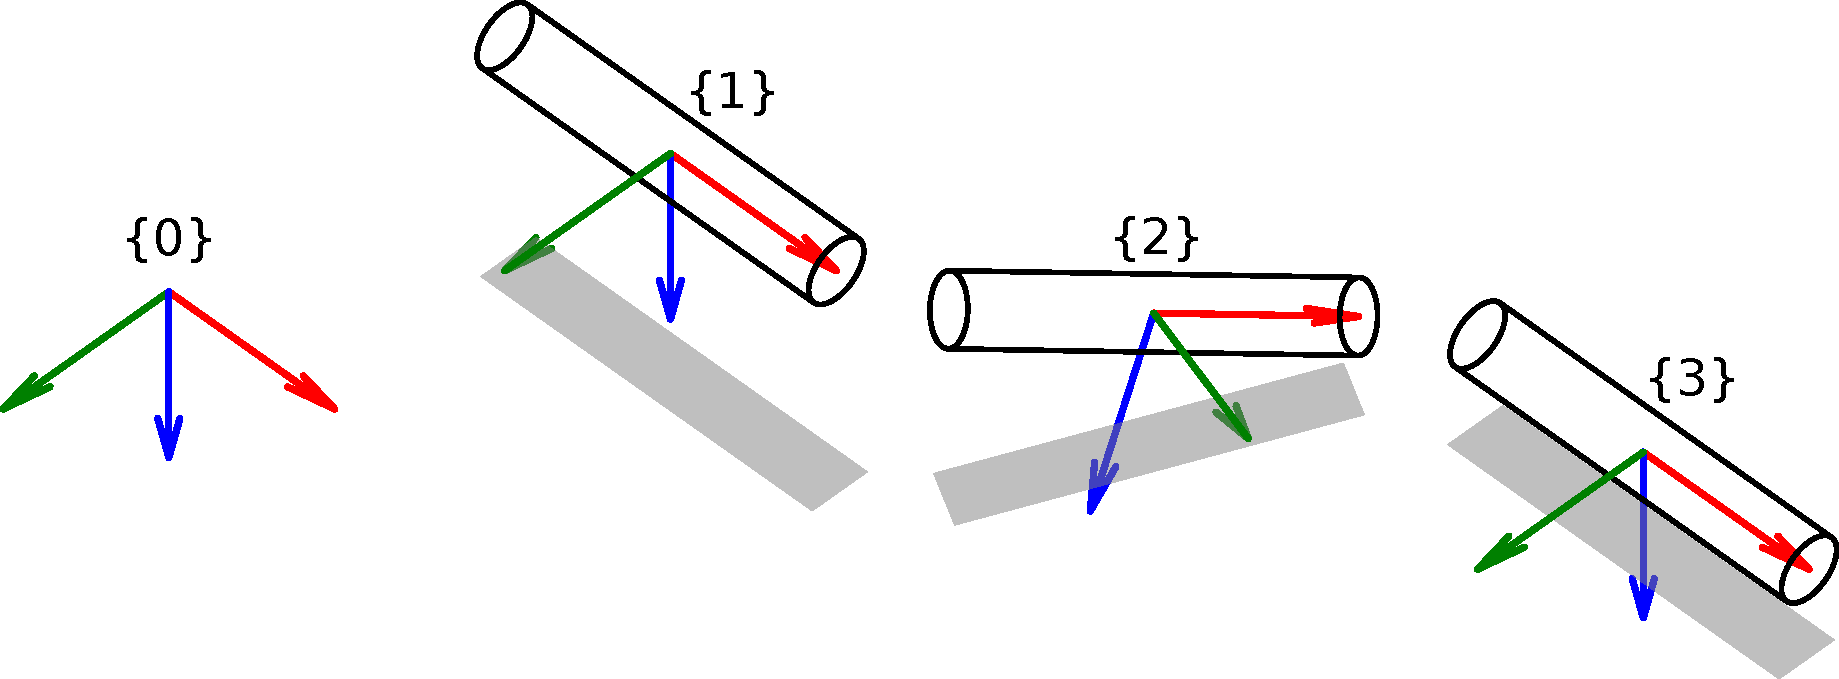
\includegraphics[width=\textwidth]{assets/frames_thin.pdf}
    \caption{Frames attached to the links of a snake-like robot.}
    \label{fig:frames}
\end{figure}
We denote some inertial \gls{ned} frame by $\{0\}$, and associate a frame to each link,
setting the frame number the same as the link number.
\autoref{fig:frames} shows an example of such a setup. Here, the system has
three links connected by two joints. To highlight the importance of the $\{0\}$-
and $\{n\}$-frames, they will also be reffered to as the $\{n\}$, for \gls{ned}, and
$\{b\}$, for body, respectively. The numbering and lettering will be used interchangeably
depending on the context.

A common way to describe the configuration of the base link is by the \gls{ned}
position and a set of Euler angles. Alterneatively, the rotation of the base link
can be described by a unit quaternion. It will be assumed that the transformations
between links are functions of a vector of joint angles, where we define
$n_j \in \mathbb{N}$ to be the total number of joint angles. Putting this together,
the necessary variables to describe the configuration of the entire system are
collected in the vector $\bm{\xi}_{\Theta} \in \R^{6+n_j}$:
%we define the configuration of the entire system as $\bm{\xi} \in \R^{6+n_j}$:
\begin{align}
    \bm{\xi}_{\Theta} &= \begin{bmatrix}\bm{\eta}_{\Theta} \\ \bm{\theta} \end{bmatrix} &
        \bm{\eta}_{\Theta} &= \begin{bmatrix}\bm{p}_{nb}^n \\ \bm{\Theta}_{nb} \end{bmatrix} &
            \bm{p}_{nb}^n &= \begin{bmatrix}x^n \\ y^n \\ z^n \end{bmatrix} &
                \bm{\Theta}_{nb} &= \begin{bmatrix}\phi \\ \theta \\ \psi \end{bmatrix} &
                    \bm{\theta} &= \begin{bmatrix}\bm{\theta}_1 \\ \vdots \\ \bm{\theta}_{n-1}\end{bmatrix},
\end{align}
where $\bm{\eta} \in \R^6$ is a collection of the the NED position $\bm{p}_{nb}^n \in \R^3$,
and Euler angles $\bm{\Theta}_{nb} \in \R^3$, of the base
link. $\bm{\theta} \in \R^{n_j}$ is the vector of joint angles, and $\bm{\theta}_i$, $i = 1,\cdots,n-1$
is a vector of joint angles for link $i$. We note that each joint can be a function of $1$ or
more joint angles.
%In the case of a unit quaternion representation of the base link,
%rotation, the vector $\bm{\Theta}_{nb}$ is replaced by a unit quaternion $\bm{q}_b^n$.
The rotation of the base link can alternatively be represented using a unit quaternion,
in that case the vector of Euler angles $\bm{\Theta}_{nb}$ is replaces by the quaternion
$\bm{q}_b^n$.
The configuration of the system is then uniquely defined by the vector $\bm{\xi}_q \in \R^{7+n_j}$.
\begin{align}
    \bm{\xi}_q &= \begin{bmatrix}\bm{\eta}_q \\ \bm{\theta} \end{bmatrix} &
        \bm{\eta}_q &= \begin{bmatrix}\bm{p}_{nb}^n \\ \bm{q}_b^n \end{bmatrix} &
            \bm{q}_{b}^n &= \begin{bmatrix}\eta \\ \bm{\epsilon} \end{bmatrix} &
                \bm{\epsilon} &= \begin{bmatrix}\epsilon_1 \\ \epsilon_2 \\ \epsilon_3 \end{bmatrix},
\end{align}
where $\eta$ is the scalar part of the quaternion and $\bm{\epsilon} \in \R^3$ is the vector part.
The quaternion satisfies the constraint $||\bm{q}_b^n||_2 = 1$. The homogeneous
transformation matrix from the base link to the inertial frame can be expressed as
\begin{align}
    \bm{H}_1^0(\bm{\eta}_{\Theta}) &= \begin{bmatrix}
        \bm{R}_b^n(\bm{\Theta})& \bm{p}_{nb}^n \\
        \bm{0}_{1\times3} & 1
    \end{bmatrix} &
    \bm{H}_1^0(\bm{\eta}_{q}) &= \begin{bmatrix}
        \bm{R}_b^n(\bm{q}_{b}^n)& \bm{p}_{nb}^n \\
        \bm{0}_{1\times3} & 1
    \end{bmatrix},
    \label{eq:H1}
\end{align}
using Euler angles and unit quaternion, respectively. In the case of Euler angles,
$\bm{R}_b^n$ uses the $x$-, $y$- and $z$-axis rotation matrices:
\begin{align}
    \bm{R}_b^n(\bm{\Theta}_{nb}) &= \bm{R}_z(\psi) \bm{R}_y(\theta) \bm{R}_x(\phi),
\end{align}
as defined in \autoref{eq:bp:so3:rotations}. Explicitly, the rotation matrix $\bm{R}_b^n$
is given by
\begin{subequations}
\begin{align}
    \bm{R}_b^n(\bm{\Theta}) &= \begin{bmatrix}
        c\psi\, c\theta & -s\psi\, c\phi + c\psi\, s\theta\, s\phi & s\psi\, s\phi + c\psi\, c\phi\, s\theta \\
        s\psi\, c\theta & c\psi\, c\phi + s\psi\, s\theta\, s\phi & -c\psi\,s\phi + s\psi\, c\phi\, s\theta \\
        -s\theta & c\theta\, s\phi & c\theta\, c\phi
    \end{bmatrix} \\
    \bm{R}_b^n(\bm{q}_b^n) &= \begin{bmatrix}
        1 - 2(\epsilon_2^2 + \epsilon_3^2) & 2(\epsilon_1\epsilon_2 - \epsilon_3\eta) & 2(\epsilon_1\epsilon_3 + \epsilon_2\eta) \\
        2(\epsilon_1\epsilon_2 + \epsilon_3\eta) & 1 - 2(\epsilon_1^2 + \epsilon_3^2) & 2(\epsilon_2\epsilon_3 - \epsilon_1\eta) \\
        2(\epsilon_1\epsilon_3 - \epsilon_2\eta) & 2(\epsilon_2\epsilon_3 + \epsilon_1\eta) & 1 - 2(\epsilon_1^2 + \epsilon_2^2)
    \end{bmatrix},
\end{align}
\end{subequations}
where $c$ and $s$ are abbreviations for the $\cos$ and $\sin$ functions, respectively. The body
frame twist $\bm{\nu}_{nb}^b$ can be found by means of \autoref{eq:def_twist}:
\begin{align}
    \label{eq:modeling:body_twist}
    \bm{\nu}_{nb}^b &= \bm{H}_b^n(\bm{\eta})^{-1} \dot{\bm{H}}_b^n(\bm{\eta}).
\end{align}
Using \autoref{eq:modeling:body_twist}, it can be shown that the body twist can be expressed
as a matrix-vector product with the state vector $\bm{\xi}$. Thist holds when $\bm{H}_b^n$ is parameterized by Euler angles,
as well as when it is parameterized by unit quaternions. The body twist
$\bm{\nu}_{nb}^b \in \R^6$ of the base link as well as the joint velocities
$\dot{\bm{\theta}} \in \R^{n-1}$ are collected in the vector $\bm{\zeta} \in \R^{6+n_j}$:
\begin{align}
    \bm{\zeta} &= \begin{bmatrix}\bm{\nu}_{nb}^b \\ \dot{\bm{\theta}}\end{bmatrix} &
        \bm{\nu}_{nb}^b = \begin{bmatrix} \bm{v}_{nb}^b \\ \bm{\omega}_{nb}^b\end{bmatrix}. 
\end{align}
Using this collection of variables,
the previously defined vectors, and \autoref{eq:modeling:body_twist}, 
the differential kinematics of the system can be expressed as \cite{fossen2021}:
\begin{subequations}
\label{eq:mod:jac}
\begin{align}
    \dot{\bm{\xi}}_{\Theta} &= \bm{J}_{\Theta}(\bm{\Theta}_{nb})\bm{\zeta} &
    \bm{J}_{\Theta}(\bm{\Theta}_{nb}) &= \begin{bmatrix}
        \bm{R}_{b}^n(\bm{\Theta}_{nb}) & \bm{0}_{3 \times 3} & \bm{0}_{3 \times n_j} \\
        \bm{0}_{3 \times 3} & \bm{T}_{b}^n(\bm{\Theta}_{nb}) & \bm{0}_{3 \times n_j} \\
        \bm{0}_{n_j \times 3} & \bm{0}_{n_j \times 3} & \I_{n_j}
    \end{bmatrix} \\
    \dot{\bm{\xi}}_{q} &= \bm{J}_{q}(\bm{q}_{b}^n)\bm{\zeta} &
    \bm{J}_{q}(\bm{q}_{b}^n) &= \begin{bmatrix}
        \bm{R}_{b}^n(\bm{q}_{b}^n) & \bm{0}_{3 \times 3} & \bm{0}_{3 \times n_j} \\
        \bm{0}_{4 \times 3} & \bm{T}_{b}^n(\bm{q}_{b}^n) & \bm{0}_{4 \times n_j} \\
        \bm{0}_{n_j \times 3} & \bm{0}_{n_j \times 3} & \I_{n_j}
    \end{bmatrix}.
\end{align}
\end{subequations}
The $\bm{T}_b^n$ matrix transforms the body fixed angular velocities to the derivative of the
rotation parameters and is given by \cite{fossen2021}:
\begin{subequations}
    \begin{align}
        \bm{T}_b^n(\bm{\Theta}_{nb}) &= \begin{bmatrix}
            1 & \sin\phi \tan\theta & \cos \phi \tan \theta \\
            0 & \cos \phi & -\sin\phi \\
            0 & \sin \phi / \cos \theta & \cos \phi / \cos \theta
        \end{bmatrix} \\
        \bm{T}_b^n(\bm{q}_{b}^n) &= \frac{1}{2}\begin{bmatrix}
            -\epsilon_1 & -\epsilon_2 & -\epsilon_3 \\
            \eta & -\epsilon_3 & \epsilon_2 \\
            \epsilon_3 & \eta & -\epsilon_1 \\
            -\epsilon_2 & \epsilon_1 & \eta
        \end{bmatrix}
    \end{align}
\end{subequations}

\iffalse
Where $\bm{R}_{nb}(\bm{\Theta}_{nb})$ is the rotation matrix from the body-fixed frame to the NED frame
using the Euler angles $\bm{\Theta}_{nb}$ as described in \autoref{sec:bp:so3_se3}.
The $\bm{T}_{nb}(\bm{\Theta}_{nb})$ matrix transforms the body fixed angular velocities
of the base link to the derivative of the Euler angles and is given by \cite{fossen2021}:
\begin{align}
    \bm{T}_{nb}(\bm{\Theta}_{nb}) = \begin{bmatrix}
        1 & \sin\phi \tan\theta & \cos \phi \tan \theta \\
        0 & \cos \phi & -\sin\phi \\
        0 & \sin \phi / \cos \theta & \cos \phi / \cos \theta
    \end{bmatrix}.
\end{align}

\begin{align}
    \bm{H}_1^0(\bm{\eta}) &= \begin{bmatrix}
        \bm{R}_z(\psi) \bm{R}_y(\theta) \bm{R}_x(\phi) & \bm{p}_{nb}^b \\
        \bm{0}_{1\times3} & 1
    \end{bmatrix} &
    \bm{p}_{nb}^b = \begin{bmatrix}x^n \\ y^n \\ z^n \end{bmatrix},
\end{align}

where $\phi$, $\theta$ and $\phi$ are the Euler angles, $x^n$, $y^n$ and $z^n$
is the position of the base link in the \gls{ned}-frame , collected
int the vector $\bm{\theta} \in \R^{n_j}$:
\fi

 



% -----------------------------------------------------------------------------
\subsection{Forward Kinematics}
\label{sec:forward_kinematics}
% 
The goal of this subchapter is to express the relations between velocities in
the previously defined frames. The most important takeaway will
be the defintion of the link-jacobians, which will be very usefull when expressing
the dynamics of a general \gls{aiauv}.
Let
\begin{align}
    \bm{H}_i^j = \begin{bmatrix}
        \bm{R}_i^j & \bm{p}_{ji}^i \\
        \bm{0}^T & 1
    \end{bmatrix} \in \SE,
\end{align}
be the homogeneous transformation matrix from frame $i$, attached to link $i$,
to frame $j$. Define
\begin{align}
    \bm{A}_i(\bm{\theta}_i) &\in \SE & i &= 1, 2, \ldots, n-1
\end{align}
as the transformation matrix from frame $i+1$ to frame $i$ such that
\begin{align}
    \bm{H}_{i+1}^k &= \bm{H}_i^k \bm{A}_i(\bm{\theta}_i). \label{eq:mod:Hi}
\end{align}
Before generalizing the joint transformations to be functions of an arbitrary number of parameters,
it will be asumed that they are functions of one variable, more specifically,
\begin{align}
    \bm{A}_i(\theta_i) &= \bm{A}_i(0) \exp(\theta_i[\bm{a}_i]_{\wedge}) & \bm{A}_i(0) &\in \SE & \bm{a}_i&\in \R^6
\end{align}
We define the body twist $\bm{\nu}_i$ of link $i$ as
\begin{align}
    [\bm{\nu}_i]_{\wedge} := [\bm{\nu}_{ni}^i]_{\wedge} := (\bm{H}_i^b)^{-1}(\dot{\bm{H}}_i^b)
\end{align}
and note that
\begin{align}
    \bm{\nu}_1 &= \bm{\nu}_{nb}^b = \bm{J}_1 \bm{\zeta} &
    \bm{J}_1 &= \begin{bmatrix}\I_{6} & \bm{0}_{n_1\times6}\end{bmatrix}
\end{align}
It turns out that the body twist of link $i+1$ can be recursively calculated from
the previous links twist:
\begin{subequations}
    \label{eq:H_recursive}
\begin{align}
    [\bm{\nu}_{i+1}]_{\wedge} &= (\bm{H}_{i+1}^b)^{-1}(\dot{\bm{H}}_{i+1}^b) \\
    &= (\bm{H}_{i}^b\bm{H}_{i+1}^i)^{-1}(\dot{\bm{H}_{i}^b\bm{H}_{i+1}^i}) \\
    &= (\bm{H}_{i}^b\bm{A}_i)^{-1}(\dot{\bm{H}_{i}^b\bm{A}_i}) \\
    &= (\bm{A}_i)^{-1}(\bm{H}_{i}^b)^{-1}(\dot{\bm{H}}_{i}^b\bm{A}_i + \bm{H}_{i}^b\dot{\bm{A}}_i) \\
    &= (\bm{A}_i)^{-1}[\bm{\nu}_i]_{\wedge}\bm{A}_i + \dot{\theta}_i[\bm{a}_i]_{\wedge} \\
    &= [\Ad^{-1}(\bm{A}_i)\bm{\nu}_i]_{\wedge} + [\dot{\theta}_i\bm{a}_i]_{\wedge} \label{eq:eta:induction}\\
    \bm{\nu}_{i+1} &= \Ad^{-1}(\bm{A}_i)\bm{\nu}_i + \dot{\theta}_i\bm{a}_i \\
    &= \Ad^{-1}(\bm{A}_i)\bm{J}_i\bm{\zeta} + \begin{bmatrix}\bm{0}_{6\times6+(i-1)} & \bm{a}_i & \bm{0}_{6\times n_j-i}\end{bmatrix}\bm{\zeta},
\end{align}
\end{subequations}
where the dependencies of the matrices are dropped for sake of brevity.
The step after \autoref{eq:eta:induction} is valid through an argument of induction, and
implicity defines the $\bm{J}_i(\bm{\theta})$ matrices.
By inspection of \autoref{eq:H_recursive}, we can conclude that
\begin{subequations}
\begin{align}
    \bm{\nu}_{i+1} &= \bm{J}_{i+1}(\bm{\theta}) \bm{\zeta} \\
    \bm{J}_{i+1}(\bm{\theta}) &= 
    \Ad^{-1}(\bm{A}_i(\bm{\theta}))\bm{J}_i\left(\bm{\theta}\right) + \begin{bmatrix}\bm{0}_{6\times6+(i-1)} & \bm{a}_i & \bm{0}_{6\times n_j-i}\end{bmatrix}.
        \label{eq:recursive_link_jacobians}
\end{align}
\end{subequations}
The matrices $\bm{J}_i(\bm{\theta})$ are important for control purposes and for expressing the 
dynamics of the system. They are reffered to as the link jacobians. It will also 
be usefull to differentiate them when doing task-priority control. Differentiating
\autoref{eq:recursive_link_jacobians} with respect to time, we get
\begin{align}
    \dot{\bm{J}}_1(\bm{\theta}) &= \bm{0}_{6\times(6+n)} \\
    \dot{\bm{J}}_{i+1}(\bm{\theta}) &= -\ad(\bm{a}_i)\bm{J}_{i+1}(\bm{\theta})\dot{\theta}_i +
        \Ad^{-1}(\bm{A}_i(\theta_i))\dot{\bm{J}}_i(\bm{\theta},\dot{\bm{\theta}})
\end{align}
It is important no note that in the general case, $\bm{\theta}_i$ is a vector of
joint parameters, not a scalar. The parameters will uniquely describe the transformation from one link
to another. We will assume that every transformation matrix $\bm{A}_i(\bm{\theta}_i)$ consits of $l_i \in \N$ transformations
of zero or one variable.
\begin{align}
    \bm{A}_i(\bm{\theta}_i) = \bm{B}_{i,1} \bm{B}_{i,2} \cdots \bm{B}_{i,l_i}.
\end{align}
For instance, the transformation $\bm{A}_1(\bm{\bm{\theta}_1}) = \bm{H}_2^1(\bm{\theta})$
in \autoref{fig:frames} can be written as the following sequance of transforms;
translation along the x-axis, rotation about the y-axis, rotation about the z-axis, and finally,
a translation along the x-axis. This can be seen in \autoref{fig:transforms_all}, where the shape
attached to the axis represents where the coordinate origin is.
\begin{figure}[h!]
    \centering
    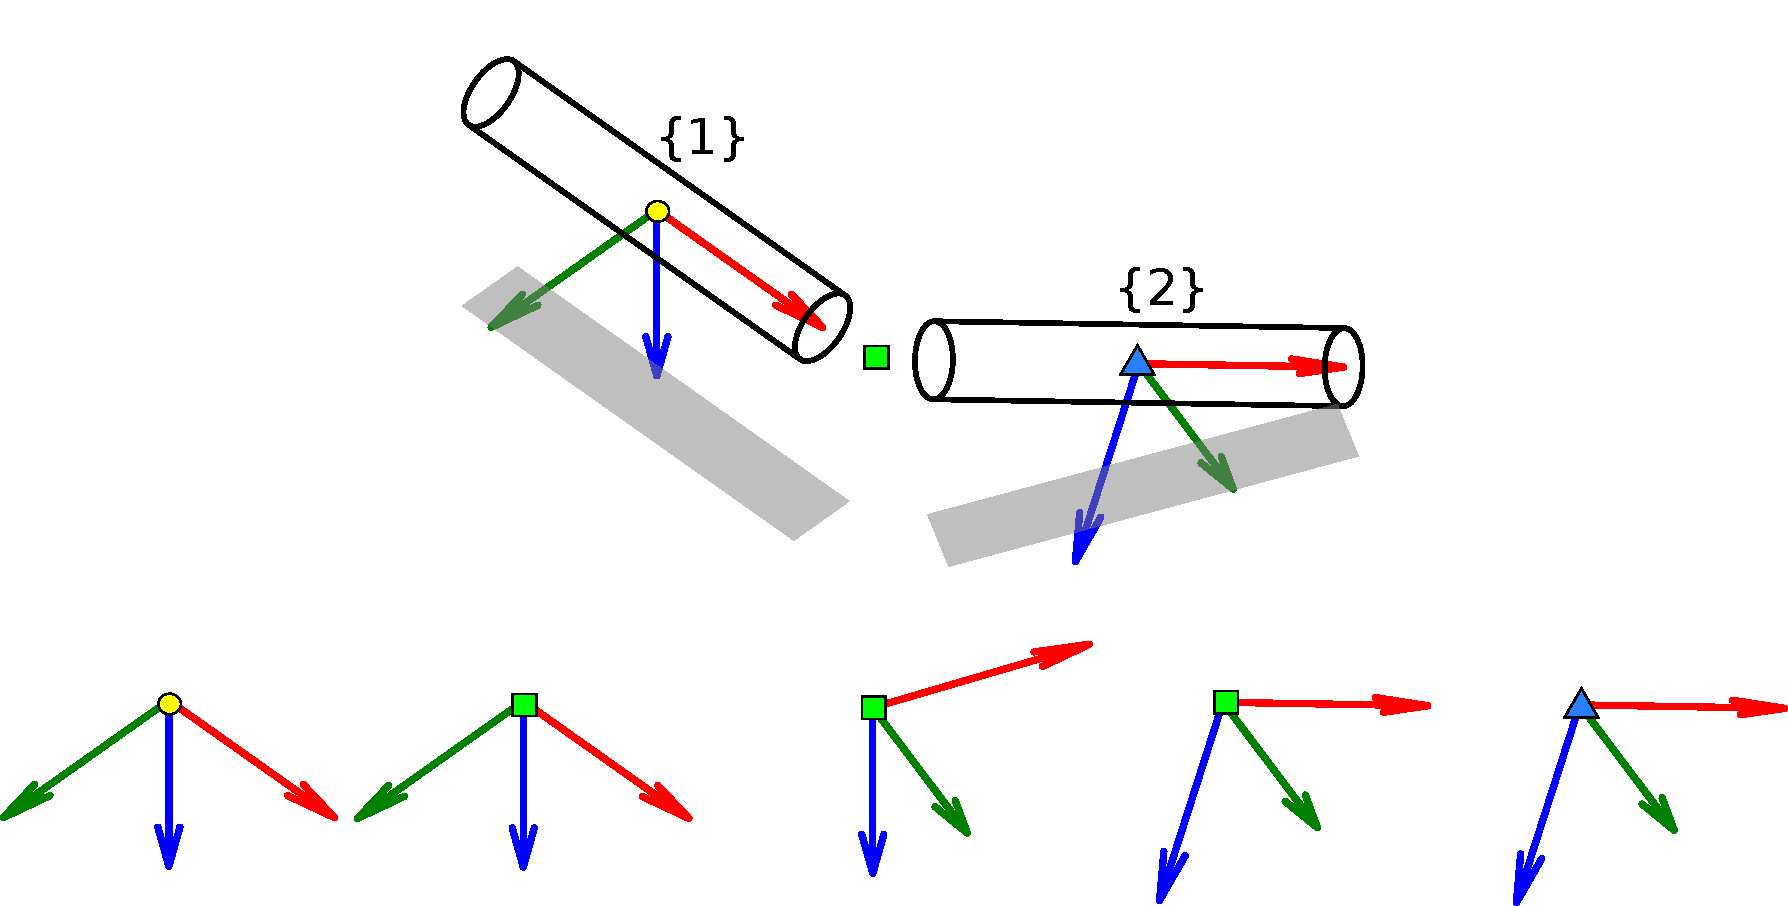
\includegraphics[width=\textwidth]{assets/transforms_all.pdf}
    \caption{Intermediate frames between frame $1$ and $2$.}
    \label{fig:transforms_all}
\end{figure}
It will be assumed that all the $\bm{B}_{i,j}(\theta)$ transformations can be written as
\begin{align}
    \bm{B}_{i,j}(0)\exp\left(\theta[\bm{b}_{i,j}]_{\wedge}\right),
\end{align}
where $\bm{b}_{i,j} \in \R^6$ is a constant vector. It it important to note that
this simple form can represent a lot of transformations in $\SE$. For instance,
a constant transform can be expressed by setting $\bm{b}_{i,j} = \bm{0}$ and choosing $\bm{B}_{i,j}(0)$.
Pure rotations of one variable can be parameterized using angle-axis parameters, using $\bm{b}_{i,j} =
\begin{bmatrix}\bm{0}^T & \bm{k}^T &\end{bmatrix}^T$, where $\bm{k}$ is the axis. Translations
are acheived by setting $\bm{b}_{i,j} = \begin{bmatrix} \bm{k}^T & \bm{0}^T \end{bmatrix}^T$.
More complex transforms, such as the one between frame $2$ and $1$ in \autoref{fig:transforms_all}
are acheived by consecutive transformations on this form. To illustrate this point, the transformation
from frame $2$ to frame $1$ in \autoref{fig:transforms_all} can be expressed as
\begin{align}
    \begin{bmatrix}1 & 0 & 0 & l_1 \\ 0 & 1 & 0 & 0 \\ 0 & 0 & 1 & 0 \\ 0 & 0 & 0 & 1\end{bmatrix}
    \exp\left(\theta_1\begin{bmatrix}\bm{0} \\ 0 \\ 0 \\ 1\end{bmatrix}_{\wedge}\right)
    \exp\left(\theta_2\begin{bmatrix}\bm{0} \\ 0 \\ 1 \\ 0\end{bmatrix}_{\wedge}\right)
    \begin{bmatrix}1 & 0 & 0 & l_2 \\ 0 & 1 & 0 & 0 \\ 0 & 0 & 1 & 0 \\ 0 & 0 & 0 & 1\end{bmatrix}.
\end{align}
Althoug the system has become much more general by allowing joint transformations to
be functions of an arbitrary number of parameters, computation of the link jacobians can
be done in a very similar way as previously shown. This is because the sequence of
transforms from frame $i+1$ to $i$ is parameterized in exactly the same way as
from $n$ to $1$ when the robot has joints of one parameter.

% ----------------
\iffalse
We define $\bm{\theta} = \begin{bmatrix}\theta_1 & \theta_2 & \cdots & \theta_{n-1}\end{bmatrix}^T$
and
\begin{align}
    \bm{A}_{i:j}(\bm{\theta}) =
    \begin{cases}
        \bm{A}_i(\theta_i) \bm{A}_{i+1}(\theta_{i+1}) \cdots \bm{A}_{j-1}(\theta_{j-1}) & i \leq j \\
        \bm{0}_{4 \times 4} & i > j \\
    \end{cases}.
\end{align}
It can be shown that the transformation matrix $\bm{A}_{i}(\theta_i)$ can be
expressed as \cite{murray2017}:
\begin{align}
    \bm{A}_i(\theta_i) &= \bm{A}_i(0) \exp([\bm{a}_i]_{\wedge} \theta_i), \label{eq:expmap}
\end{align}
for some $\bm{a}_i \in \R^6$. The body twist
of link $i+1$ relative to the inertial frame $n$ can be expressed as
\begin{subequations}
\begin{align}
    \bm{\nu}_{n(i+1)}^{i+1} &= \left(\bm{H}_{i+1}^n\right)^{-1} \dot{\bm{H}}_{i+1}^n \\
    &= \bm{A}_{1:i}^{-1}(\bm\theta) \bm{H}_1^{-1} \dot{\bm{H}}_{1} \bm{A}_{1:i}(\bm\theta) \nonumber \\
    &+ \bm{A}_{2:i}^{-1}(\bm\theta) [\bm{a}_1]_{\wedge}\bm{A}_{2:i}(\bm\theta) \dot{\theta}_1 \nonumber \\
    &\vdots \label{eq:body_twist_def} \\
    &+ \bm{A}_{i:i}^{-1}(\bm\theta) [\bm{a}_{i-1}]_{\wedge}\bm{A}_{i:i}(\bm\theta) \dot{\theta}_{i} \nonumber \\
    &+ [\bm{a}_{i}]_{\wedge} \dot{\theta}_i. \nonumber
\end{align}
\end{subequations}
Defining $\bm{\nu}_i := \bm{\nu}_{ni}^i$ as the body twist of link $i$ relative to
the inertial frame $n$, \autoref{eq:body_twist_def} can be written recursively as:
\begin{subequations}
    \label{eq:body_twist_recursive}
\begin{align}
    \bm{\nu}_{1} &= \bm{\nu}_{n1}^1 \\
    \bm{\nu}_{i+1} &= \Ad^{-1}(\bm{A}_i(\theta_i)) \bm{\nu}_i + [\bm{a}_i]_{\wedge} \dot{\theta}_i.
\end{align}
\end{subequations}
This motivates the definition of the link Jacobians that are defined in a way
such that
\begin{align}
    \bm{\nu}_{i} = \bm{J}_i(\bm{\theta}) \bm{\zeta}
\end{align}
where the body twist $\bm{\nu}$ and the joint velocities $\dot{\bm{\theta}}$ are
collected in the vector $\bm{\zeta}$:
\begin{align}
    \bm{\zeta} = \begin{bmatrix}\bm{\nu} \\ \dot{\bm{\theta}}\end{bmatrix} \in \R^{6+(n-1)}.
\end{align}
From \autoref{eq:body_twist_recursive} we can see that the link Jacobians can be
defined as
\begin{subequations}
    \label{eq:link_jacobian}
\begin{align}
    \bm{J}_1(\bm{\theta}) &= \begin{bmatrix} \bm{I}_6 & \bm{0}_{6 \times n} \end{bmatrix} \\
        \bm{J}_{i+1}(\bm{\theta}) &= \begin{bmatrix}
            \Ad^{-1}(\bm{A}_{1:i}(\bm{\theta}))  &  \Ad^{-1}(\bm{A}_{2:i}(\bm{\theta})) \bm{a}_1 &
            \cdots & \bm{a}_i & \bm{0}_{6 \times (n-i)}
        \end{bmatrix} \\
    &= \Ad^{-1}(\bm{A}_i(\theta_i)) \bm{J}_i(\bm{\theta}) + \begin{bmatrix}
        \bm{0}_{6 \times (5+i)} & \bm{a}_i & \bm{0}_{6 \times (n-i)}
    \end{bmatrix}.
\end{align}
\end{subequations}
The derivatives of the link Jacobians are needed for control purposes and
calculation of the Coriolis matrix. By differentiating \autoref{eq:link_jacobian}
with respect to time, we get
\begin{subequations}
\begin{align}
    \dot{\bm{J}}_1(\bm{\theta}) &= \bm{0}_{6\times(6+n)} \\
    \dot{\bm{J}}_{i+1}(\bm{\theta},\dot{\bm{\theta}}) &= -[\bm{a}_i]_{\wedge} \Ad^{-1}(\bm{A}_i(\theta_i))
        \bm{J}_i(\bm{\theta})\dot{\theta}_i + \Ad^{-1}(\bm{A}_i(\theta_i))\dot{\bm{J}}_i(\bm{\theta},\dot{\bm{\theta}}) \\
    &= -[\bm{a}_i]_{\wedge}\bm{J}_{i+1}(\bm{\theta})\dot{\theta}_i +
        \Ad^{-1}(\bm{A}_i(\theta_i))\dot{\bm{J}}_i(\bm{\theta},\dot{\bm{\theta}}).
\end{align}
\end{subequations}

\fi %--------------------------


\subsection{Dynamics}

For each link, $i$, defined in the previous subchapter, we associate the following
properties: $\bm{M}_i \in \R^{6 \times 6}$ is the inertia matrix of the link,
$\bm{J}_i \in \R^{6 \times (6+n)}$ is the link jacobian, $\bm{C}_i \in \R^{6 \times 6}$
is the Coriolis matrix, $\bm{D}_i \in \R^{6 \times 6}$ is the damping matrix and
$\bm{g}_i \in \R^{6}$ is the gravitational forces and hydrostatic forces and moments.
The damping matrix will be discussed in \autoref{sec:hydrodynamics}.
$\bm{M}_i$ takes into account the added mass of the link
\begin{align}
    \bm{M}_i &= \bm{M}_{RB,i} + \bm{M}_{A,i},
\end{align}
where $\bm{M}_{RB,i}$ is the rigid body inertia matrix of the link and $\bm{M}_{A,i}$
is the added mass matrix of the link. As a result of the added mass, the Coriolis
matrix is given by
\begin{align}
    \bm{C}_i &= \bm{C}_{RB,i} + \bm{C}_{A,i}
\end{align}
where $\bm{C}_{RB,i}$ is the Coriolis matrix of the rigid body and $\bm{C}_{A,i}$
is a function of the added mass matrix. The added mass matrix and the damping matrix
for each link is the topic of \autoref{sec:hydrodynamics}. The dynamics of the
system described in the previous subchapter can be modeled as
\cite{from2014}:
\begin{align}
    \bm{M}(\bm{\theta})\dot{\bm{\zeta}} +
        \bm{C}(\bm{\theta}, \bm{\zeta}) \bm{\zeta} +
        \bm{D}(\bm{\theta}, \bm{\zeta}) \bm{\zeta} +
        \bm{g}(\bm{\xi}) =
        \bm{\tau}.
\end{align}
$\bm{M}(\bm{\theta}) \in \R^{(6+n)\times(6+n)}$  is the inertia matrix of the
system, $\bm{C}(\bm{\theta}, \bm{\zeta}) \in \R^{(6+n)\times(6+n)}$ is the
Coriolis matrix, $\bm{D}(\bm{\theta}, \bm{\zeta}) \in \R^{(6+n)\times(6+n)}$ is
the damping matrix, $\bm{g}(\bm{\xi}) \in \R^{6+n}$ is the gravitational forces
and buoyancy forces and moments acting on the system, $\bm{\tau} \in \R^{n}$ is the generalized
forces acting on the system as a result of the actuators,
and $\bm{\tau}_{\mathrm{ext}} \in \R^{6+n}$ is the
generalized external forces acting on the system. Let $\bm{J}_{i}(\bm{\theta})$
be the link Jacobians as defined in \autoref{eq:link_jacobian}.
The inertia matrix
can be expressed as
\begin{align}
    \bm{M}(\bm{\theta}) &= \sum_{i=1}^{n} \bm{J}_{i}^T(\bm{\theta}) \bm{M}_i \bm{J}_{i}(\bm{\theta}).
\end{align}
Note that if the Jacobians are full rank, the inertia matrix is positive definite.
Furthermore, it is always symmetric. The Coriolis matrix can be expressed as
\begin{align}
    \bm{C}(\bm{\theta}, \bm{\zeta}) &=
    \sum_{i=1}^{n} \bm{J}_{i}^T(\bm{\theta}) \bm{M}_i \dot{\bm{J}}_{i}(\bm{\theta},\dot{\bm{\theta}})
    -\bm{J}_{i}^T(\bm{\theta}) \bm{C}_i(\bm{\theta},\bm{\zeta})_i \bm{J}_{i}(\bm{\theta}) \bm{\zeta}.
\end{align}
The damping matrix can be expressed as
\begin{align}
    \bm{D}(\bm{\theta}, \bm{\zeta}) &=
    \sum_{i=1}^{n} \bm{J}_{i}^T(\bm{\theta}) \bm{D}_i(\bm{\theta},\bm{\zeta}) \bm{J}_{i}(\bm{\theta}).
\end{align}
and the gravitational forces and buoyancy forces and moments can be expressed as
\begin{align}
    \bm{g}(\bm{\xi}) &=
    \sum_{i=1}^{n} \bm{J}_{i}^T(\bm{\theta}) \bm{g}_i(\bm{\xi}).
\end{align}
The control inputs $\bm{u}$ are mapped to the generalized forces $\bm{\tau}$ by
the actuator configuration matrix $\bm{B}(\bm{\theta})$ as
\begin{align}
    \bm{\tau} &= \bm{B}(\bm{\theta}) \bm{u} &
    \bm{B}(\bm{\theta}) &= \begin{bmatrix}
        \bm{J}_1^T(\bm{\theta}) \bm{B}_1 & \cdots & \bm{J}_n^T(\bm{\theta}) \bm{B}_n
    \end{bmatrix},
\end{align}
where $\bm{B}_i$ is the actuator configuration matrix for link $i$. For a simple
thruster configuration, such as in the case where all thrusters are fixed with
respect to some link, the $\bm{B}_i$ matrices are constant and can be expressed
as
\begin{align}
    \bm{B}_i &= \begin{bmatrix}
        \bm{\beta}_{t,i,1} & \cdots & \bm{\beta}_{t,i,m} \\
        \bm{r}_{t,i,1} \times \bm{\beta}_{t,i,1} & \cdots & \bm{r}_{t,i,m} \times \bm{\beta}_{t,i,m}
    \end{bmatrix},
\end{align}
where $\bm{\beta}_{t,i,j}$ is the direction of the thrust and $\bm{r}_{t,i,j}$
is the point of application of the thrust.





% -----------------------------------------------------------------------------
\section{Hydrodynamics}
\label{sec:hydrodynamics}

Hydrodynamics is the study of the forces acting on a body in a fluid. The forces
can be modeled as potential forces, giving rise to the added mass matrix, and
damping forces. This chapter will focus on how to model the hydrodynamic forces
acting on a rigid body in a fluid.

\subsection{Added Mass}

When a rigid body accelerates in a fluid, the fluid is accelerated as well. 
This contributes to the total kinetic energy of the system \cite{antonelli2018}.
To account for these effects, the spatial inertia matrix of the rigid body
can be augmented to approximate the total kinetic energy of the system: 
\begin{equation}
    \bm{M} = \bm{M}_{RB} + \bm{M}_{A}.
\end{equation}
The matrix $\bm{M}_A$ is in reality a function of the wave excitation frequency
of the waves in the ocean \cite{fossen2021}. Because of the complex computations
of $\bm{M}_A(\omega)$, as well as the fact that for large vessels the natural
frequencies of the vessel are much lower than the wave excitation frequencies,
the added mass matrix is approximated as the zero-frequency added mass matrix
\begin{align}
    \bm{M}_A(\omega) &\approx \bm{M}_A(0)
\end{align}
Under this assumption, the kinetic energy of the fluid $T_A$ is approximated
as
\begin{align}
    T_a &= \frac{1}{2}\bm{\nu}^T\bm{M}_A\bm{\nu} & \dot{\bm{M}}_A &= \bm{0},
\end{align}
where $\bm{\nu}$ is the twist velocity of the rigid body. For underwater 
vehicles at low speed where the the shape has three planes of symmetry, the
added mass matrix can be approximated as \cite{fossen2021}:
\begin{align}
    \bm{M}_A = \bm{M}_A^T =
    -\operatorname{diag}(X_{\dot{u}}, Y_{\dot{v}}, Z_{\dot{w}},
        K_{\dot{p}}, M_{\dot{q}}, N_{\dot{r}}).
\end{align}
According to \cite{fossen2021} this approximation is found to be quite good for
many applications due to the fact that the off diagonal coupling terms are small
compared to the diagonal terms.

By applying strip theory the added mass matrix for a cylindrical rigid body of
mass $m$, length along the x-axis $l$ and radius $r$ can be derived as \cite{fossen1994}:
\begin{align}
 X_{\dot{u}} &= -0.1 m &
 Y_{\dot{v}} &= -\pi \rho r^2 l \nonumber \\
 Z_{\dot{w}} &= -\pi \rho r^2 l &
 K_{\dot{p}} &= 0 \\
 M_{\dot{q}} &= -\frac{1}{12} \pi \rho r^2 l^3 &
 N_{\dot{r}} &= -\frac{1}{12} \pi \rho r^2 l^3 \nonumber
\end{align}
where $\rho$ is the density of the fluid. For a three-dimensional ellipsoid with
lengths $a$, $b$ and $c$ along the x, y and z axis respectively, the added mass
can be approximated as \cite{fossen2021}:
\begin{align}
 X_{\dot{u}} &= -\frac{\alpha_0}{2-\alpha_0}m &
 Y_{\dot{v}} &= -\frac{\beta_0}{2-\beta_0}m \nonumber \\
 Z_{\dot{w}} &= Y_{\dot{v}}&
 K_{\dot{p}} &= 0 \label{eq:ellipsoid_added_mass} \\
 M_{\dot{q}} &= -\frac{1}{5}\frac{(b^2-a^2)^2(\alpha_0-\beta_0)}{2(b^2-a^2) + (b^2+a^2)(\beta_0-\alpha_0)}m&
 N_{\dot{r}} &= M_{\dot{q}} \nonumber
\end{align}

\subsection{Damping}

There are several phenomena that contribute to the damping of a rigid body in
a fluid. Among these are potential damping, skin friction, wave drift damping,
damping due to vortex shedding and lifting forces. In many cases
all of these effects can be approximated using a linear damping matrix $\bm{D}$ and
a quadratic damping matrix $\bm{D}_n$ \cite{fossen2021}. Damping can be modeled
as
\begin{align}
    \bm{D}(\bm{\nu}_r) &= \bm{D} + \bm{D}_n(\bm{\nu}_r) \\
    \bm{\tau}_d &= \bm{D}(\bm{\nu}_r)\bm{\nu}_r
\end{align}
for a 6-DOF rigid body, $\bm{D}(\bm{\nu}_r)$ is a $6\times 6$ matrix, $\bm{\nu}_r$
is the twist of the rigid body relative to the fluid and $\bm{\tau}_d \in \R^6$
is a vector of the damping forces and moments acting on the rigid body. \cite{antonelli2018}
states that the damping matrix can be approximated as
\begin{subequations}
\begin{align}
    \bm{D} &= -diag(X_u, Y_v, Z_w, K_p, M_q, N_r) \\
    \bm{D}_n &= -diag(X_{u|u|}|u|, Y_{v|v|}|v|, Z_{w|w|}|w|, K_{p|p|}|p|, M_{q|q|}|q|, N_{r|r|}|r|),
\end{align}
\end{subequations}

for completely submerged bodies. This will neglect coupling and dissipative effects.
It has been shown that by using strip theory, the damping force and
moment on a cylinder can be approximated by the follwing integrals \cite{mcmillan1995}:
\begin{subequations}
    \label{eq:cylinder_damping}
    \begin{align}
        \bm{f}_d &= - \rho C_D r \int_{0}^{l} ||\bm{v}^n(x)|| \bm{v}^n(x) \,dx \\
        \bm{m}_d &= - \rho C_D r \int_{0}^{l} ||\bm{v}^n(x)||
        \left(\begin{bmatrix}x & 0 & 0\end{bmatrix}^T \times \bm{v}^n(x)\right) \,dx,
    \end{align}
\end{subequations}
where $r$ and $l$ are the radius and length of the cylinder, $\rho$ the density
of the fluid, $C_D$ the drag coefficient and $\bm{v}^n(x)$ the velocity of the
fluid at the point $x$ along the length of the cylinder. Using the results stated
in \autoref{eq:cylinder_damping}, \citeauthor{schmidt2018} proposes a linear
damping matrix for a cylinder as \cite{schmidt2018}:
\begin{align}
    \bm{D} = \rho \pi l C_D v_{ref}
    \begin{bmatrix}
        \beta &            0 &             0 &          0 &              0 &            0 \\
            0 &            1 &             0 &          0 &              0 & \frac{1}{2}l \\
            0 &            0 &             1 &          0 &  -\frac{1}{2}l &            0 \\
            0 &            0 &             0 & \gamma r^2 &              0 &            0 \\
            0 &            0 & -\frac{1}{2}l &          0 & \frac{1}{3}l^2 &            0 \\
            0 & \frac{1}{2}l &             0 &          0 &              0 & \frac{1}{3}l^2
    \end{bmatrix},
\label{eq:damping_cyl}
\end{align}
where $C_D$, $v_{ref}$, $\beta$, $\gamma$ are constants to be determined.

% -----------------------------------------------------------------------------
\iffalse
\section{UVMS Kinematics}

The following chapter will descibe the kinematics of an \gls{uvms}
The \gls{uvms} consists of a rigid base and is connected to
a manipulator with $n$ links. This makes the \gls{uvms} have a snake-like structure.
Adopting notation from \cite{fossen2021}, the rigid base can be uniquely described
by a set of $6$ coordinates
\begin{align}
    \bm{\eta} &= \begin{bmatrix} \bm{p} \\ \bm{\Theta} \end{bmatrix} \in \R^6 &
        \bm{p} &= \begin{bmatrix} x^n \\ y^n \\ z^n \end{bmatrix} \in \R^3 &
    \bm{\Theta} &= \begin{bmatrix} \phi \\ \theta \\ \psi \end{bmatrix} \in \R^3,
\end{align}
where $\bm{p}$ is the position of the base described in a NED frame and $\bm{\Theta}$
are the Euler angles describing the orientation of the base. Note that the Euler
angles are singular at $\theta = \pm \pi/2$, and that using quaternions
would avoid this problem. Introducing quaternions would however add an extra
equality constraint to the system, making the system harder to simulate. Because
of this, Euler angles are used in this thesis. 

We assume the position of the manipulator links relative to the base are uniquely
described by a set of $n$


% -----------------------------------------------------------------------------
\section{UMS Dynamics}



% mention that the damping matrix is a function of the velocity of the body
% mention that for UVMs the damping matrix can be assumed decoupled for all links.

{
    \color{red}
    \begin{itemize}
        \item Multi-body dynamics
        \item Hydrodynamics (damping)
        \item Jacobians
        \item Inspiration from Henrik?
    \end{itemize}
}
\fi

\chapter{Task-Priority Control}
\label{chap:tpc}

This chapter explores various methods for task priority control, beginning with
an introduction to its fundamental concepts and a presentation of one of the
earliest and most straightforward techniques. It then continues into more advanced
approaches and concludes with a discussion of key implementation considerations,
including singularity robustness, for real-world robotic applications.

% -----------------------------------------------------------------------------
\section{Introduction}
\label{sec:tpc_intro}

Task priority control addresses the problem of managing multiple objectives simultaneously in a robotic system. It is a widely used methodology for handling redundancy in robots, enabling them to perform several tasks at once without compromising the executing of higher-priority objectives. Understanding the concept of tasks, their prioritization, and how multiple tasks interact is essential for understanding the fundamentals of task priority control.

A task refers to a specific objective or goal that a robotic system aims to achieve. Tasks can represent a wide variety of objectives, such as moving an end-effector to a desired position and orientation, maintaining a specific posture, avoiding joint limits, preventing collisions, or controlling specific velocities or accelerations at specific points. The tasks are typically described using functions, which map system states to task-specific outputs. These outputs are then often compared to desired values to determine the error and guide the control system towards achieving the task.

The prioritization of tasks is a key aspect of task-priority control. When a task is assigned a higher priority, it must be executed without being disturbed or compromised by lower-priority tasks. This means that the control system must balance the objectives of multiple tasks, ensuring that the higher-priority tasks are achieved while still allowing the lower-priority tasks to be executed. In practice, higher priority tasks are resolved first, and the remaining degrees of freedom are used to achieve the lower-priority tasks. For example, a robotic manipulator tasked with avoiding obstacles might prioritize obstacle avoidance over maintaining an exact end-effector position.

\sloppy{
In the following sections, we will develop the mathematical foundations of task-priority control, exploring the concepts of kinematic- and dynamic-level task-priority control.
}

% -----------------------------------------------------------------------------
\section{Kinematic-level Redundancy Resolution}

Kinematic-level redundancy resolution is a fundamental concept in task-priority control.
It is one of the first methods proposed for handling redundancy in a task-priority framework.
A fundamental assumption in kinematic-level redundancy resolution is that there
already exists a controller that can generate the desired generalized velocities \(\bm{\zeta}_d(t)\).
Considerations around this assumption will be discussed in later sections.
The mathematical concepts introduced in this section are presented in introductory
chapters in many of the articles and books on task-priority control, such as
\cite{hanafusa1981}, \cite{nakamura1987}, \cite{khatib1987}. An overview is
presented in \cite{chiaverini1997}.

\subsection{Velocity-level control}
\label{sec:velocity_level_control}

A task variable $\bm{\sigma}(t) \in \mathbb{R}^m$ is defined as a function of the robot's
state $\bm{\xi}(t) \in \mathbb{R}^n$:
\begin{align}
    \bm{\sigma}(t) = \bm{f}(\bm{\xi}(t)) \label{eq:def_task}.
\end{align}
A task can then be defined as the objective of keeping the task variable $\bm{\sigma}(t)$
close to a desired value $\bm{\sigma}_d(t) \in \mathbb{R}^m$. For instance, a task could
be the end-effector position of a robot manipulator or the orientation of a camera mounted
on a robot. By differentiating \autoref{eq:def_task} with respect to time, the task velocity
can be defined as
\begin{align}
    \dot{\bm{\sigma}}(t) = \frac{\partial \bm{f}(\bm{\xi}(t))}{\partial \bm{\xi}}
    \dot{\bm{\xi}}(t)= \left(\frac{\partial \bm{f}(\bm{\xi}(t))}{\partial \bm{\xi}}
    \bm{J}_{\Theta/q}(\bm{\xi}(t)) \right)\bm{\zeta}(t) \label{eq:def_task_jacobian},
\end{align}
where \(\bm{J}_{\Theta/q}\) describes the relation between \(\bm{\xi}\) and \(\bm{\zeta}\)
as shown in \autoref{eq:mod:jac}. It is important no note that this jacobian is dependent
on the parametrization choosen for the orientation; quaternion or Euler angles.
Collecting the parenthesis of \autoref{eq:def_task_jacobian} in a matrix
\(\bm{J}(\bm{\xi}(t))\), we get the following relation;
\begin{align}
    \dot{\bm{\sigma}}(t) = \bm{J}(\bm{\xi}(t))\bm{\zeta}(t).
\end{align}
The matrix \(\bm{J}(\bm{\xi}(t)) \in \mathbb{R}^{n \times m}\) is called the
\emph{task Jacobian}, or simply the \emph{Jacobian}, and maps the generalised
velocities $\bm{\zeta}(t)$ to the task velocity $\dot{\bm{\sigma}}(t)$.
The Jacobian is a function of the robot's state \(\bm{\xi}(t)\).
In the case where only one task is considered, one can use the pseudoinverse
to compute the minimum norm generalized velocities that will achieve the desired
task velocity. The generalized velocities are then given by
\begin{align}
    \bm{\zeta}_d(t) = \bm{J}^{+}(\bm{\xi}(t)) \dot{\bm{\sigma}}_d(t) \label{eq:task_priority}
\end{align}
where \(\bm{J}^{+}(\bm{\xi}(t))\) is the pseudoinverse of the Jacobian at the current
state \(\bm{\xi}(t)\). From now on the dependencies of $\bm{J}$, \(\bm{\xi}\)
and $\bm{\sigma}$ will be omitted for brevity.

In practice, the Jacobian might not represent the true kinematics of the robot.
Furthermore, depending on the task, the desired task velocity might not be feasible,
and there might be model errors and noise in the estimated generalized velocities making
the generalized velocities not equal to the desired generalized velocities. Because of this,
a feedback controller is needed to ensure that the desired task velocity is
achieved. Substituting the desired task velocity \(\dot{\bm{\sigma}}_d(t)\) in 
\autoref{eq:task_priority} with
a feedforward term and a feedback term, the generalized velocities can be computed as
\begin{align}
    \bm{\zeta}_d = \bm{J}^{+} \left(\dot{\bm{\sigma}}_d + \bm{\Lambda}\tilde{\bm{\sigma}}\right),
\end{align}
where $\tilde{\bm{\sigma}} = \bm{\sigma} - \bm{\sigma}_d$ is the error in the
task and the constant matrix $\bm{\Lambda}$ is a matrix that determines the
feedback gains.
Generalizing this to multiple tasks, we note that \autoref{eq:def_task_jacobian}
has a more general solution than \autoref{eq:task_priority} when $n > m$:
\begin{align}
    \bm{\zeta}_d = \bm{J}^{+} \dot{\bm{\sigma}}_d + (\mathbb{I} - \bm{J}^{+} \bm{J}) \bm{z},
\end{align}
for some arbitrary vector $\bm{z} \in \mathbb{R}^n$. The term
$(\mathbb{I}_n - \bm{J}^{+} \bm{J}) \bm{z}$ is recognized as the null space projection
of $\bm{z}$ onto the null space of the Jacobian matrix $\bm{J}$. By setting
$\bm{z}$ to some desired value, such as the generalized velocities of a lower-priority task,
one can achieve prioritization of tasks. To present the basic idea, consider the
tasks
\begin{subequations}
\begin{align}
    \bm{\sigma}_i &= \bm{f}_i(\bm{\xi}) \in \mathbb{R}^{m_i} &i &= 1, 2, \ldots, k \\
    \dot{\bm{\sigma}}_i &= \bm{J}_i(\bm{\xi}) \bm{\zeta} \in \mathbb{R}^{m_i} &i &= 1, 2, \ldots, k
\end{align}
\end{subequations}
with corresponding desired tasks
\begin{align}
    \dot{\bm{\sigma}}_{i,d}(t) \quad i = 1, 2, \ldots, k
\end{align}
Let $\bm{N}_i = \mathbb{I}_n - \bm{J}_i^{+} \bm{J}_i$ be the null space projection
matrix onto the null space of the Jacobian $\bm{J}_i$.
The desired generalized velocities are then given by
\begin{align}
    \bm{\zeta}_d = \sum_{i=1}^k \bm{N}_i^{\#}\bm{J}_i^{\#} \left(\dot{\bm{\sigma}}_{i,d} + \bm{\Lambda}_i \tilde{\bm{\sigma}}_i\right) \label{eq:task_priority_vel}
\end{align}
comparing this to the single task case, $\bm{N}_i^{\#}$ is the null space projection matrix
projecting a task onto the null space of all the higher-priority tasks.
\begin{align}
    \bm{N}_i^{\#} = \bm{N}_1 \bm{N}_2 \cdots \bm{N}_{i-1}
\end{align}
and the $\bm{J}_i^{\#}$ matrix is the projection matrix projecting a task onto the
subspace spanned by the task Jacobian.
\begin{align}
    \bm{J}_i^{\#} = \bm{J}_i^+
\end{align}
In general, several slightly different task priority control frameworks have
been proposed, following the same basic form as \autoref{eq:task_priority_vel}.
Although, slight variations in the form of the null space projection matrices
and the pseudoinverse matrices have been proposed. The methods include substituting
the pseudoinverse with the transpose of the Jacobian, and using augmented null space
projections.
The augmented null space projection is defined as
\begin{subequations}
    \label{eq:augmented_null_space}
\begin{align}
    \bm{N}_i^{\#} := \bm{N}_{1\cdots i-1} := \mathbb{I} - \bm{J}_{1\cdots i-1}^+ \bm{J}_{1\cdots i-1} \\
    \bm{J}_{1\cdots i-1} := \begin{bmatrix}
        J_1 \\
        J_2 \\
        \vdots \\
        J_{i-1}
    \end{bmatrix}
\end{align}
\end{subequations}
This gives rise to several different variants of the task priority control algorithm.
The variants discussed in \cite{antonelli2009} are summarized in the following table:
\begin{table}[h]
    \centering
    \begin{tabular}{|c|c|c|}
        \hline
        $J^{\#}$ & $N^{\#}$ & Algorithm's name \\
        \hline
        $\bm{J}^+$ & $\bm{N}_1 \bm{N}_2 \cdots \bm{N}_{i-1}$ & successive inverse-based projections \\
        $\bm{J}^+$ & $\bm{N}_{1\cdots i-1}$ & augmented inverse-based projections \\
        $\bm{J}^T$ & $\bm{N}_1 \bm{N}_2 \cdots \bm{N}_{i-1}$ & successive transpose-based projections \\
        $\bm{J}^T$ & $\bm{N}_{1\cdots i-1}$ & augmented transpose-based projections \\
        \hline
    \end{tabular}
    \label{tab:tpc_variants}
    \caption{Task priority control variants. Table from \cite{antonelli2009}}
\end{table}

Using the successive method, task velocities are progressively projected into the null space of higher-priority tasks by recursively multiplying null space projection matrices. In contrast, the augmented method constructs a single null space projection matrix by stacking the task Jacobians of all higher-priority tasks and then computing the pseudoinverse of this stacked matrix. This distinction is illustrated in \autoref{eq:augmented_null_space}.
It is important to emphasize that these two approaches are not equivalent. Null space projection matrices are generally not commutative, which means the successive method can yield a more conservative null space projection, whereas the augmented method often results in a less conservative projection, offering increased flexibility for lower-priority tasks.
From a computational perspective, the successive method is typically more efficient because it recursively computes the null space projection matrices. Conversely, the augmented method demands the computation of the pseudoinverse of a potentially large stacked Jacobian matrix, which is computationally more intensive.

% -----------------------------------------------------------------------------
\subsection{Acceleration-level control}

The previous chapter discusses the velocity-level control of tasks. It is also 
possible to determine the double derivative of the state variables corresponding to some
desired task acceleration. This is referred to as acceleration-level control.
To see this, consider \autoref{eq:def_task_jacobian} and differentiate
with respect to time once more:
\begin{align}
    \ddot{\bm{\sigma}} = \frac{d}{dt}\left(\bm{J} \bm{\zeta}\right) = \dot{\bm{J}} \bm{\zeta} + \bm{J} \dot{\bm{\zeta}}
    \label{eq:task_acc_jacobian}
\end{align}
Solving this equation for the derivative of the generalized velocities \(\dot{\bm{\zeta}}\) gives
\begin{align}
    \ddot{\bm{q}} = \bm{J}^{+} \left(\ddot{\bm{\sigma}} - \dot{\bm{J}}\dot{\bm{q}}\right) +
    \left(\mathbb{I} - \bm{J}^{+}\bm{J}\right) \bm{z} \label{eq:task_acc_control},
\end{align}
for some arbitrary vector $\bm{z} \in \mathbb{R}^n$. Inspired from the
velocity-level control, one can define the desired joint accelerations as
\begin{align}
    \ddot{\bm{q}}_d = \bm{J}^{+} \left(\ddot{\bm{\sigma}}_d
    - \dot{\bm{J}}\dot{\bm{q}}\right) \label{eq:task_priority_acc}.
\end{align}
One can impose the closed-loop characteristic of the task by defining the desired
task acceleration implicitly as
\begin{align}
    \left(\ddot{\bm{\sigma}}_d - \ddot{\bm{\sigma}}\right) +
    \bm{K}_d\left(\dot{\bm{\sigma}}_d - \dot{\bm{\sigma}}\right) +
    \bm{K}_p\left(\bm{\sigma}_d - \bm{\sigma}\right) = 0 \label{eq:task_acc}
\end{align}
where $\bm{K}_d$ and $\bm{K}_p$ are positive definite matrices. Substituting
\autoref{eq:task_acc} into the desired joint accelerations \autoref{eq:task_acc_jacobian},
and doing this for each task, one can get the desired joint accelerations:
\begin{subequations}
\begin{align}
    \bm{J}_i\ddot{\bm{q}} &= -\dot{\bm{J}}_i\dot{\bm{q}} + \ddot{\bm{\sigma}}_{i,d} 
    + \bm{K}_{d,i}\left(\dot{\bm{\sigma}}_{i,d} - \dot{\bm{\sigma}}_i\right)
    + \bm{K}_{p,i}\left(\bm{\sigma}_{i,d} - \bm{\sigma}_i\right) \\
    &=: \bm{h}_i(\bm{q}, \dot{\bm{q}}, t) \\
    \ddot{\bm{q}}_d &= \bm{J}_1^{+} \bm{h}_1 + \left(\mathbb{I} - \bm{J}_1^+\bm{J}_1\right) \bm{J}_2^{+} \bm{h}_2.
\end{align}
\end{subequations}
This method is called acceleration-level task priority control. The method can
be generalized to multiple tasks by using the same methods as presented in \autoref{sec:tpc_intro}.


\subsection{Low level control}

{
\color{red}
\begin{itemize}
    \item Add citations
    \item Decoupling of the quaternion vector in control
    \item Include chapter about set-based TPC
    \item Include chapter about how task-jacobians can be created.
\end{itemize}
}

The methods discussed above assume the existence of a controller capable of tracking the desired joint velocities \(\bm{\zeta}_d\). This implies that a lower-level controller must be designed and implemented, and its performance will directly affect the ability to follow the specified tasks.

A straightforward approach to tracking the desired generalized velocities is to use a simple \gls{pd} controller. However, because the robot’s state includes a unit quaternion and the generalized velocities are defined in the body frame—while the robot's state itself is defined in the \gls{ned} frame—some care must be taken during controller design. The controller can be written as:

\begin{subequations}
\label{eq:tau_pd}
\begin{align}
    \begin{bmatrix}
        \bm{p}_{nb,d}^n & {\bm{q}_{b,d}^n}^T & {\bm{\theta}_d}^T
    \end{bmatrix}^T
    &:=
    \bm{\xi}_{q,d}(t) := \int_{0}^{t} \bm{J}_q(\bm{q}_b^n(\tau))\bm{\zeta}_d(\tau)\,d\tau
    \\
    \begin{bmatrix} \eta_e & \bm{\varepsilon}_e^T\end{bmatrix}^T &:= \left(\bm{q}_{b,d}^n\right)^* \otimes \bm{q}_b^n
    \\
    \bm{\tau}_{PD} &= 
    \bm{K}_p \begin{bmatrix}
        \bm{R}_b^n(\bm{q}_b^n)^T\left(\bm{p}_{nb,d}^n - \bm{p}_{nb}^n\right) \\
        -\sgn{(\eta_e)} \bm{\varepsilon}_e \\
        \bm{\theta}_d - \bm{\theta}
    \end{bmatrix} + 
    \bm{K}_d  \left(\bm{\zeta}_d - \bm{\zeta} \right), 
\end{align}
\end{subequations}

where \(\bm{\tau} \in \R^{10}\) denotes the desired generalized forces on the body. The desired state \(\bm{\xi}_d\) is obtained by integrating the desired generalized velocities \(\bm{\zeta}_d\). The remaining symbols are defined in \autoref{sec:diff_kin}.

It's important to note that this controller does not account for low-frequency disturbances such as waves, ocean currents, or hydrodynamic forces. These will introduce low-frequency tracking errors. However, this limitation is mitigated by the higher-level, velocity-based task-priority controller, which includes feedback that adapts the desired velocity based on state error.

Minor improvements to the controller can still be made. While modeling the full dynamics of an \gls{aiauv} is challenging, gravity and buoyancy forces can be accurately captured if the vehicle’s mass and volume distributions are known. This leads to an extended controller, referred to as \gls{pd}+, which augments the original controller from \autoref{eq:tau_pd} with a compensation term:

\begin{align}
    \bm{\tau}_{PD+} = \bm{\tau}_{PD} + \bm{g}(\bm{\xi}(t)),
\end{align}

where \(\bm{g}(\bm{\xi}(t))\) is defined in \autoref{eq:modeling:g}. Provided the gravity and buoyancy forces are modeled correctly, this addition improves the steady-state tracking error, particularly in the vertical (downward) direction.

% -----------------------------------------------------------------------------
\newpage
\section{Dynamic-level Redundancy Resolution}
\label{sec:tpc:dynamic_level}

Dynamic-level redundancy resolution solves the redundancy problem by considering
the robot's dynamics. This removes the need for a controller that can generate
the desired joint velocities $\dot{\bm{q}}_d(t)$, and instead uses the robot's
dynamic model to generate a generalized torque $\bm{\tau}_d(t)$ that will
be applied to the robot. There are several methods for dynamic-level redundancy
resolution, but here we will focus on the method presented in \cite{khatib2004}.
Consider the robot's dynamic model similar to models presented in previous sections:
\begin{subequations}
\begin{align}
    \bm{M}(\bm{q}) \ddot{\bm{q}} + \bm{N}(\bm{q}, \dot{\bm{q}}) \dot{\bm{q}} + \bm{g}(\bm{q}) &= \bm{\tau} \\
    \bm{q}, \dot{\bm{q}} ,\ddot{\bm{q}},\bm{\tau} &\in \mathbb{R}^n.
\end{align}
\end{subequations}
In the equation above, $N(\bm{q}, \dot{\bm{q}})$ represents the Coriolis and
damping forces acting on the robot. We consider a case with $2$ tasks, $\bm{\sigma}_t$
and $\bm{\sigma}_p$, and the corresponding Jacobians $\bm{J}_t$ and $\bm{J}_p$.
The essential equations concerning the tasks are:
\begin{subequations}
    \begin{align}
        \dot{\bm{\sigma}}_t &= \bm{J}_t(\bm{q}) \dot{\bm{q}} & \dot{\bm{\sigma}}_p &= \bm{J}_p(\bm{q}) \dot{\bm{q}} \\
        \ddot{\bm{\sigma}}_t &= \bm{J}_t(\bm{q}) \ddot{\bm{q}} + \dot{\bm{J}}_t(\bm{q}) \dot{\bm{q}} &
        \ddot{\bm{\sigma}}_p &= \bm{J}_p(\bm{q}) \ddot{\bm{q}} + \dot{\bm{J}}_p(\bm{q}) \dot{\bm{q}}.
    \end{align}
\end{subequations}
We define a dynamically consistent generalized inverse \cite{khatib1987} as
\begin{subequations}
    \begin{align}
        \bar{\cdot} &: \R^n \times \R^{m\times n} \rightarrow \R^{m\times n} & m &= 1, \cdots, n\\
        \bar{\cdot} &: (\bm{q},\bm{X}) \mapsto \bm{M}^{-1}(\bm{q})\bm{X}^T\left(
            \bm{X}\bm{M}^{-1}(\bm{q})\bm{X}^T.
        \right)^{-1}
    \end{align}
\end{subequations}
The dynamically consistent generalized inverse is used to project the system dynamics
onto the task space. For the sake of brevity, the dependencies of $\bm{q}$ and $\bm{\sigma}$
will be omitted in the following equations. We define the following properties and
select the applied generalized force $\bm{\tau}$ as
\begin{align}
    \bm{N}_t &:= \I - \bar{\bm{J}}_t \bm{J}_t &
    \bm{J}_{p|t} &:= \bm{J}_p \bm{N}_t &
    \bm{\tau} = \bm{J}_t^T \bm{f}_t + \bm{J}_{p|t}^T \bm{f}_p,
    \label{eq:force_application}
\end{align}
where $\bm{f}_t$ and $\bm{f}_p$ are forces applied in task space to be
specified. To build some intuition, consider the projected dynamics onto
the two task spaces, slightly abusing notation:
\begin{subequations}
    \label{eq:projected_dynamics}
\begin{align}
    \bar{\bm{J}}_t^T \left[
        \bm{M} \ddot{\bm{q}} + \bm{N} \dot{\bm{q}} + \bm{g} = \bm{\tau}
        \right]
    &\Rightarrow
    \bm{\Lambda}_t \ddot{\bm{\sigma}}_t + \bm{\mu}_t + \bm{p}_t = \bm{f}_t \\
    \bar{\bm{J}}_{p|t}^T \left[
        \bm{M} \ddot{\bm{q}} + \bm{N} \dot{\bm{q}} + \bm{g} = \bm{\tau}
        \right]
    &\Rightarrow
    \bm{\Lambda}_{p|t} \ddot{\bm{\sigma}}_p + \bm{\mu}_{p|t} + \bm{p}_{p|t} = \bm{f}_{p|t},
\end{align}
\end{subequations}
where
\begin{subequations}
\begin{align}
    \bm{\Lambda}_t &:= \left(\bm{J}_t \bm{M}^{-1} \bm{J}_t^T\right)^{-1} &
    \bm{\mu}_t &:= \bar{\bm{J}}_t^T \bm{N} \dot{\bm{q}} &
    \bm{p}_t &:= \bar{\bm{J}}_t^T \bm{g} \\
    \bm{\Lambda}_{p|t} &:= \left(\bm{J}_{p|t} \bm{M}^{-1} \bm{J}_{p|t}^T\right)^{-1} \label{eq:lambda_pIt} &
    \bm{\mu}_{p|t} &:= \bar{\bm{J}}_{p|t}^T \bm{N} \dot{\bm{q}} &
    \bm{p}_{p|t} &:= \bar{\bm{J}}_{p|t}^T \bm{g}
\end{align}
\end{subequations}
This is assuming that the Jacobians are full rank, implying that the task-space
mass matrices are invertible. From \autoref{eq:projected_dynamics}, it is clear
that one can use a feedback linearization technique to control the tasks. By
choosing the forces $\bm{f}_t$ and $\bm{f}_{p|t}$ as
\begin{subequations}
\begin{align}
    \bm{f}_t &= \bm{\Lambda}_t \bm{f}_t^* + \bm{\mu}_t + \bm{p}_t \\
    \bm{f}_{p|t} &= \bm{\Lambda}_{p|t} \left(\bm{f}_p^* - \ddot{\bm{\sigma}}_{\overline{p|t}}\right) + \bm{\mu}_{p|t} + \bm{p}_{p|t} \label{eq:osc_fp|t}\\
    \ddot{\bm{\sigma}}_{\overline{p|t}} &:= \ddot{\bm{\sigma}}_p - \ddot{\bm{\sigma}}_{p|t},
\end{align}
\end{subequations}
one can achieve the desired task accelerations $\bm{f}_t^*$ and
$\bm{f}_p^*$. The term $\bm{J}_t^T\bm{f}_t$ in \autoref{eq:force_application} can induce an acceleration in the 
controllable $p$-space, this is compensated for by the
$\ddot{\bm{\sigma}}_{\overline{p|t}}$ term \cite{sentis2004}:
\begin{align}
    \ddot{\bm{\sigma}}_{\overline{p|t}} = \bm{J}_p \bm{M}^{-1} \bm{J}_t^T \bm{f}_t
    + \bm{\Lambda}_{p|t}^{-1}\left(\bm{\mu}_{p|t} + \bm{p}_{p|t}\right)
    - \bm{\Lambda}_{p}^{-1}\left(\bm{\mu}_p + \bm{p}_p\right)
\end{align}
Assuming that the tasks are compatible, the desired task accelerations can be
shown to be
\begin{align}
    \ddot{\bm{\sigma}}_t &= \bm{f}_t^* & \ddot{\bm{\sigma}}_p &= \bm{f}_p^*.
\end{align}
In the case where $\bm{J}_{p|t}\bm{M}^{-1}\bm{J}_{p|t}^T$ in \autoref{eq:lambda_pIt}
is singular, the task-space mass matrix $\bm{\Lambda}_{p|t}$ can be generalized
as the Moore-Penrose pseudoinverse of the matrix \cite{khatib2004}:
\begin{align}
    \underline{\bm{\Lambda}}_{p|t} &:= \left(\bm{J}_{p|t} \bm{M}^{-1} \bm{J}_{p|t}^T\right)^{+} &
    \label{eq:lambda_pIt_pseudo}
\end{align}
Substituting $\bm{\Lambda}_{p|t}$ in \autoref{eq:osc_fp|t} with
$\underline{\bm{\Lambda}}_{p|t}$ in \autoref{eq:lambda_pIt_pseudo} allows for
accelerations in the non-conflicting directions in the $p$-space.

The method presented above has been generalized to multiple tasks in \cite{sentis2004}.
This will not be discussed in this thesis, but the essence of the method is the same
as presented above.

% -----------------------------------------------------------------------------
\section{Singularity Robustness}
\label{sec:tpc:sing_robust}

Considerations have to be taken into account when implementing the
pseudoinverse numerically on a computer. One of the most important considerations is the singularity
robustness of the algorithm. Although the pseudoinverse is defined for all matrices,
when the matrix is close to being singular, the pseudoinverse can be very sensitive
to small changes in the matrix. This might lead to very large input torques along
almost-singular directions. This problem is discussed extensively in \cite{chiaverini1997}.
The following section will discuss the singularity robustness of the algorithm used in this
thesis as proposed by \cite{chiaverini1997}.

First, consider the problem of taking the pseudoinverse of an arbitrary matrix $\bm{J}$.
As discussed in \autoref{sec:pseudoinverse}, the SVD of a matrix $\bm{J}$ can be
written as
\begin{align}
    \bm{J} = \bm{U} \bm{\Sigma} \bm{V}^T,
\end{align}
and the pseudoinverse of $J$ is
\begin{align}
    \bm{J}^+ = \bm{V} \bm{\Sigma}^+ \bm{U}^T.
\end{align}
Rewriting the $\bm{U}$ and $\bm{V}$ matrices as
\begin{subequations}
\begin{align}
    \bm{U} &= \begin{bmatrix} \bm{u}_1 & \bm{u}_2 & \cdots & \bm{u}_n \end{bmatrix} \\
    \bm{V} &= \begin{bmatrix} \bm{v}_1 & \bm{v}_2 & \cdots & \bm{v}_m \end{bmatrix}
\end{align}
\end{subequations}
where $\bm{u}_i$ and $\bm{v}_i$ are the columns of $\bm{U}$ and $\bm{V}$ respectively.
$\bm{J}$ and its pseudoinverse can be written as
\begin{subequations}
\begin{align}
    \bm{J} &= \sum_{i=1}^r \sigma_i \bm{u}_i \bm{v}_i^T \\
    \bm{J}^+ &= \sum_{i=1}^r \frac{1}{\sigma_i} \bm{v}_i \bm{u}_i^T.
\end{align}
\end{subequations}
From this, it is clear that when $\sigma_i$ is close to zero, the pseudoinverse
will be very sensitive to small changes in $\sigma_i$. One proposed solution to
this problem is the so-called \emph{damped pseudoinverse} which is defined as
\begin{align}
    \bm{J}^* := \sum_{i=1}^r \frac{\sigma_i}{\sigma_i^2 + \lambda^2} \bm{v}_i \bm{u}_i^T.
\end{align}
We see that for large values of $\sigma_i$,
\begin{align}
    \frac{\sigma_i}{\sigma_i^2 + \lambda^2} \approx \frac{1}{\sigma_i},
\end{align}
and for small values of $\sigma_i$,
\begin{align}
    \frac{\sigma_i}{\sigma_i^2 + \lambda^2} \approx 0.
\end{align}
This will make the pseudoinverse well-conditioned for all values of $\sigma_i$.
The trade-off is that the damped pseudoinverse will not be the true pseudoinverse.
This might lead to tasks with lower priority affecting the higher-priority tasks and
breaking some of the assumptions made when proving stability and task consistency.

A way to make the pseudoinverse more accurate when far from singularities is to
use the \emph{variable damped least-squares inverse} (VDLSI) proposed by \cite{chiaverini1997}.
This uses the fact that there is no need to damp the pseudoinverse when far from singularities.
The VDLSI is defined as
\begin{subequations}
\begin{align}
    \bm{J}^{\circ} := \sum_{i=1}^r \frac{\sigma_i}{\sigma_i^2 + \lambda_i^2(\sigma_i)} \bm{v}_i \bm{u}_i^T \\
    \lambda_i^2(\sigma_i) = \begin{cases}
        0 & ,\sigma_i \geq \varepsilon \\
        \left(1-\left(\frac{\sigma_i}{\varepsilon}\right)^2\right)\lambda_{max}^2 & ,\sigma_i < \varepsilon,
    \end{cases}
\end{align}
\end{subequations}
where $\lambda_{max}^2$ and $\varepsilon$ are parameters that can be tuned. $\lambda_{max}$
determines the maximum damping factor and $\varepsilon$ determines a threshold for when
to start damping the pseudoinverse based on how close the singular values are to zero.
To better illustrate the difference between the different methods, see \autoref{fig:1_x}
showing the LSI, VLSI and VDLSI on a scalar matrix for $\lambda=\epsilon=0.1$.

\begin{figure}[h]
    \centering
    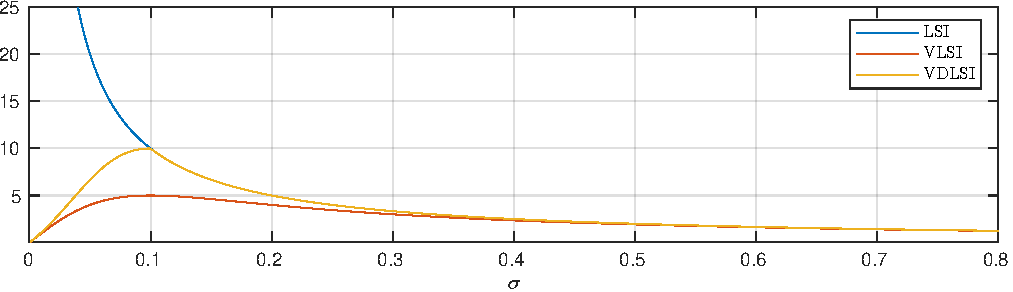
\includegraphics[width=\textwidth]{assets/singval.pdf}
    \caption{Comparison of the LSI, VLSI and VDLSI on a scalar matrix.}
    \label{fig:1_x}
\end{figure}




\chapter{Simulation}

\begin{figure}[h!]
    \centering
    \includegraphics[width=\textwidth]{assets/ignored/eely-thruster.png}
    \caption{Eelys thruster module}
    \label{fig:module:thruster}
\end{figure}


\chapter{Conclusion \& Future Work}
\label{ch:conclusion}

% ------------------------------------------------------------------ Conclusion
\section{Conclusion}

This thesis presents an experimental validation of a kinematic-level \gls{tpc} framework specifically tailored for the Eelume robot. The primary contributions and findings of this research include:
\begin{itemize}
\item \textbf{Control, Visualization, and Simulation Software}: Comprehensive control, visualization, and simulation software was developed as part of this thesis. The control software facilitates efficient implementation and testing of task-priority controllers and other controller types without requiring detailed handling of low-level communication protocols. The visualization software provides immediate, real-time overviews of experimental results, while the simulation environment enables thorough and safe testing of experimental controllers prior to deployment on the actual Eelume robot.

\item \textbf{Low-level \gls{pd+} Controller}: A robust low-level \gls{pd+} controller was designed, implemented, and experimentally verified. The controller demonstrates reliable reference tracking, exhibiting some steady-state errors primarily in depth and roll orientations.

\item \textbf{Velocity-Level \gls{tpc}}: A velocity-level \gls{tpc} controller was successfully integrated into the control software and experimentally validated. This controller effectively tracks desired tasks and consistently respects task priority constraints when managing conflicting task objectives.

\item \textbf{Set-Based \gls{tpc}}: A velocity-level \gls{tpc} controller incorporating set-based tasks, designed specifically to handle joint limitations, was implemented and validated through experiments. The results confirmed reliable tracking performance under compatible task conditions and underscored the significance of careful task design when tasks become incompatible.
\end{itemize}

% ----------------------------------------------------------------- Future Work
\section{Future Work}
\label{sec:conclusion:future_work}

While this thesis demonstrates the feasibility of kinematic-level \gls{tpc} on a lightweight, highly redundant underwater robot, several areas remain open for further exploration and development. The work presented here lays the foundation for multiple extensions and improvements, both in terms of modeling accuracy and control strategy sophistication. Potential directions for future work include:

\begin{itemize}
    \item \textbf{Model identification}: Although an approximate dynamic model was developed as part of this thesis, further improvements are needed to enhance its fidelity. In particular, accurate estimation of added mass and hydrodynamic damping remains challenging. Dedicated experimental procedures could be designed to more precisely identify these parameters, significantly improving model-based control strategies.

    \item \textbf{Dynamic-level \gls{tpc}}: A natural extension of the work presented here is the implementation of \gls{tpc} at the dynamic level. This would require a significantly more accurate dynamic model, as control inputs would be computed based on full system dynamics rather than velocity kinematics alone. With a sufficiently precise model, dynamic-level TPC may offer improved performance in terms of responsiveness and disturbance rejection.

    \item \textbf{Controller tuning}: There is considerable scope for improving performance through systematic tuning of both the low-level \gls{pd+} controller and the high-level \gls{tpc} parameters. In particular, the proportional gains for individual tasks could be better adapted to system behavior. Additionally, since the robot's local dynamics vary with configuration, implementing a gain-scheduled or adaptive control strategy could further enhance tracking performance.

    \item \textbf{Rejection of joint measurement jitter}: Joint angle jitter was partially mitigated in this thesis using low-pass filtering. However, more advanced techniques—such as outlier detection, sensor fusion, or model-based filtering—could allow for more effective rejection of faulty measurements without introducing significant time delays.

    \item \textbf{Advanced control strategies}: The software and experimental framework developed in this thesis enables further research into advanced control techniques. Methods such as adaptive control, learning-based strategies, or alternative task-priority formulations could be implemented and tested using the same platform. This opens up new avenues for exploration and motivates continued development of the system.
\end{itemize}



\printbibliography
\addcontentsline{toc}{chapter}{Bibliography}
\newpage
\appendix

\includepdf[pages=-]{./assets/ignored/KIchecklist.pdf}
\addcontentsline{toc}{chapter}{AI Checklist}

\end{document}
